%\chapter{Calibration et Performances}

%----------------------------------------------------------------------------------------
%
%   DATA REDUCTION
%
%----------------------------------------------------------------------------------------
\section{La chaîne de calibration et d'analyse des données}
\label{se:pipeline}

\subsection{La calibration}
\label{se:overview_calibration}

La calibration consiste à mesurer un ensemble de propriétés et de
paramètres des détecteurs. Elle s'articule en plusieurs étapes, qui
seront détaillées dans les sections suivantes, et qui comprennent:
\begin{itemize}
  \item{La reconstruction du pointage. Cette étape, qui présente
    des spécificités imposées par l'utilisation de matrices de KID,
    consiste à mesurer la position de chaque détecteur dans le plan
    focal par rapport à un point de référence. Cette procédure, aussi
    appelée géométrie, est décrite à la Sect.~\ref{se:fov_geometry}.}
  \item{Sélection et inter-calibration des KID. Une fois le pointage
    de chaque détecteur connu, il est possible de projeter les données
    ordonnées en temps (\emph{Time-Ordered Information}, TOI)} des KIDs
    pour former des cartes. A partir d'une observation de type
    {\tt beammap} (Sect.~\ref{se:beammap}) d'une source ponctuelle
    et brillante, des cartes individuelles de la source, telle qu'elle
    a été observée par chacun des KID, sont réalisées. Cet ensemble
    de cartes nous permet de mesurer le gain de chaque KID, réalisant
    ainsi leur inter-calibration. Nous réalisons également une
    sélection des KID en fonction d'une série de critères de qualité
    mesurés sur les cartes individuelles.
  \item{La calibration de la réponse à la transmission
    atmosphérique. La fréquence de résonance des KID varie
    proportionellement aux variations de la transmission de
    l'atmosphère (voir Sect.~\ref{se:rawdata}). En calibrant la
    relation entre
    fréquence de résonance et transmission atmosphérique, il est
    possible de mesurer l'opacité de l'atmosphère pour chaque
    observation. Cette étape est détaillée à la
    Sect.~\ref{se:opacity}.}
  \item{La calibration absolue. A partir de la mesure de l'opacité de
    l'atmosphère lors d'une observation, l'atténuation atmosphérique
    instantanée peut être estimée et corrigée, pour obtenir une mesure
    du flux. Une série de mesures du flux d'un calibrateur primaire
    (e.g. Uranus) nous permet d'estimer le coefficient de calibration
    absolue (Sect.~\ref{se:calibration})}
\end{itemize}

A l'issu de ces étapes, les résultats de la calibration sont compilés
dans un fichier unique, rassemblant toutes les informations sur les
KID. Ce fichier, appelé \emph{kidpar}, contient donc les données de
pointage, la sélection, les paramètres de réponse à l'atmosphère et
les coefficients de calibration relative (gain) et absolue de chaque
KID. Le \emph{kidpar}, qui doit être construit à chaque campagne
d'observation, est passé en entrée de la chaîne de traitement de
données développée par la collaboration NIKA2 (coordinateur: Nicolas
Ponthieu).

\subsection{L'analyse des données}
\label{se:overview_pipeline}

La chaîne d'analyse de données, ou \emph{pipeline}, permet de passer
des données brutes, telles qu'elles sont fournies en sortie de
l'acquisition de données (Sect.~\ref{se:rawdata}), à un ensemble de
cartes par matrices et par bandes de fréquence, utilisables pour
l'exploitation scientifique. La calibration elle-même s'appuie en
grande partie sur cet outil. Il s'articule donc avec la calibration en
venant lire et mettre à jour le \emph{kidpar}. Une fois la calibration
réalisée, et concrêtisée par la construction du \emph{kidpar} final,
le \emph{pipeline} est utilisé pour la caractérisation des
performances. Une description de ce \emph{pipeline} utilisé à cette
fin est donnée dans~\citet{Perotto2019}. Nous en présentons rapidement
ici les modules principaux :

\subsubsection{Production et masquage des TOI}
Les TOI des KID sont constituées de l'ensemble des mesures de la
variation des fréquences de résonance. Elles sont produites à partir
des données brutes fournies par l'acquisition suivant la méthode
décrite à la Sect.~\ref{se:rawdata}. Ensuite, sont créés des masques
afin de couper les données non-utilisables pour l'exploitation
scientifique. Tout d'abord, sont détectés les impacts de rayons
cosmiques. \'Etant donné les constantes de temps très courtes des
KID, un rayon cosmique n'affecte q'un seul échantillon de données,
qui est alors masqué. Sont également masquées, les TOI des KID exclus
de la sélection de détecteurs réalisée lors de la calibration, et
les TOI des KID bruités, définis comme les KID dont la rms du bruit
est mesurée à 3$\sigma$ au dessus de la rms médiane du bruit des
détecteurs appartenant à la même matrice.

\subsubsection{Production des TOI de pointage} Le système de contrôle du
télescope, avec lequel l'acquisition des données est synchronisée,
nous fournit une TOI de pointage d'un point de référence dans le
plan focal, qui coïncide avec le détecteur de référence après
l'analyse d'un scan de pointage (voir Sect.~\ref{se:pointing}). A
partir des positions relative des détecteurs par rapport à ce point
de référence, telles qu'elles sont stockées dans le \emph{kidpar},
nous produisons une TOI de pointage pour chacun des KID.

\subsubsection{Calibration des TOI} Les TOI brutes, en Hz, sont converties en
Jy/beam en deux étapes. Elles sont d'abord multipliées par les gains
des détecteurs, évalués à opacité atmosphérique nulle, et par le
coefficient de calibration absolue. Ensuite, elles sont corrigées de
l'atténuation de l'atmosphère sur la ligne de visée, modélisée par
$\exp{\left( \taunu \, x(t)\right)}$, où $\taunu$ est l'opacité atmosphérique
mesurée pour le scan d'observation et $x(t)$ la masse d'air
traversée pour l'élévation au temps $t$.

\subsubsection{Soustraction du bruit corrélé}
Le bruit des détecteurs est dominé par plusieurs composantes de bruit
basse-fréquence commun à plusieurs détecteurs. On parle alors de bruit
\emph{corrélé}. Le bruit corrélé inclut le bruit atmosphérique,
dominant, sauf conditions d'observation exceptionnelles, et commun à
tous les KID, et le bruit électronique, commun aux KID connectés à la
même ligne de base de l'électronique de lecture (voir
Sect.~\ref{se:matrices}). Puisqu'il est commun à plusieurs détecteurs,
il est possible d'estimer un bruit corrélé générique, un
\emph{template}, et de le soustraire aux signaux de chaque KID. Ce
processus, appélé la décorrélation du bruit, est une étape critique du
traitement des données. En effet, le résidu de bruit corrélé est l'un
des facteurs limitant la sensibilité des matrices de KID.

La décorrélation du bruit a suscitée le développement d'une série de
méthodes d'analyse dédiées. Des pistes d'amélioration sont encore à
l'étude~\citep{Ponthieu2020}. La méthode la plus simple pour construire
un template de bruit corrélé repose sur le fait que l'atmosphère,
située dans le champ proche, reste la même à chaque instant pour tous
les KID, tandis que la source, en champ lointain, est observée de
façon décalée en temps par des KID différents. Par conséquent, une
moyenne de la TOI de tous les KID préserve le bruit atmosphérique et
diminue le signal astrophysique. Un template de bruit corrélé estimé
de cette manière est un \emph{mode commun}.

Pour la caractérisation des performances, nous avons opté pour une
méthode simple et robuste, bien adaptée au traitement des objets
compacts (qui constituent la vaste majorité de nos sources de
calibration). Cette méthode, appelée \emph{Most Correlated Pixels} (MCP),
inclut deux raffinements par rapport à un simple mode commun. Tout
d'abord, la matrice de corrélation entre les détecteurs (pixels) est
évaluée afin de construire un mode commun pour chaque détecteur à
partir des TOI des KID qui lui sont le plus corrélés. Ensuite, afin de
limiter encore la contribution du signal astrophysique, seuls les KID
n'observant pas la source sont utilisés pour estimer chaque
échantillon de la TOI de bruit corrélé. Ce masquage de la source dans
l'espace temporel induit un filtrage des échelles angulaires plus
grandes que l'extension du masque. Pour l'étude de sources diffuses,
ce filtrage doit être précisément estimé et corrigé pour retrouver
l'émission étendue. En revanche, la décorrélation MCP préserve bien le
signal des sources compactes. 

\subsubsection{Création de cartes} En utilisant les données de
pointages, les TOI calibrées et débruitées de tous les KID valides
d'une même matrice sont projettées tangentiellement dans une grille
régulière sur le ciel pour former une carte de densité de flux par
matrice. La résolution des cartes est choisie suffisament haute
(typiquement 2'') pour limiter les effets de pixellisation
même en utilisant la méthode des plus proches voisins (\emph{nearest
  grid point}). Pour combiner tous les détecteurs d'une même matrice,
les TOI sont pondérées par l'inverse de la variance du bruit, celle-ci
étant évaluée à partir de la déviation standard des échantillons de
données pris loin de la source. Chaque carte de flux est accompagnée
d'une carte de variance. Celle-ci est inhomogène, dépendant de la
stratégie de balayage. De plus, le résidu de bruit corrélé
basse-fréquence à l'issu de la décorrélation induit une corrélation
des pixels de la carte. Les cartes de variance sont estimées à partir
de la déviation standard de la carte de flux évaluée loin de
la source et de la carte de coups, construite par comptage du
nombre d'échantillons par pixels de la carte. Le bruit corrélé
résiduel est pris en compte en augmentant l'incertitude sur le flux
d'un facteur variant de 1,2 à 1,5 et dont l'évaluation est décrite
dans~\citet{Perotto2019}.\\

Le \emph{pipeline} d'analyse de données, brièvement décrit
ci-dessus, a été développé d'abord pour la phase de
\emph{commissioning} de NIKA2. Il s'appuie sur l'expérience acquise
avec l'analyse des données de NIKA~\citep{Catalano2014,
  Adam2014}. Comme précédemment mentionné, il constitue l'outil de
base pour la caractérisation des
performances~\citep{Adam2018, Perotto2019, Ponthieu2020}, mais il est
aussi actuellement utilisé pour l'exploitation scientifique de
l'ensemble des données de NIKA2 au télescope de
30-m~\citep{Ruppin2018, Ruppin2019c}.  


%----------------------------------------------------------------------------------------
%
%   FOV Geometrie
%
%----------------------------------------------------------------------------------------
\section{La reconstruction du plan focal}
\label{se:fov_geometry}

Dans les matrices de KID, chaque détecteur est repéré par sa fréquence
d'excitation $f_{\rm{tone}}$ (voir Sect.~\ref{se:matrices}). La
première étape de la calibration consiste donc à relier chaque
détecteur à sa position dans le plan focal. Cette
étape, appelée reconstruction du plan focal ou géométrie, est le
préalable à toute production de cartes du ciel à partir de données
issues de KIDs.

\subsection{Caractérisation des KID}
\label{se:KID_pointing}

Pour ce faire, nous utilisons une observation de type {\tt beammap}
(voir Sect.~\ref{se:beammap}) d'une source compact et brillante, telle
Uranus ou le quasar 3C84, nous permettant de construire une carte
individuelle par KID. L'objectif étant d'estimer les données de
pointage nécessaire à l'obtention de cartes, le processus est
nécessairement itératif. A la première étape, les TOI des KIDs sont
projettées en coordonnées \emph{Nasmyth} (attachées à la cabine du
télescope) à partir des données de pointage du point de référence
fournies par le télescope. Pour chaque KID, la source n'apparait pas
au centre de la carte, mais décalée suivant la position du KID par
rapport au point de référence. C'est cette position du KID relative au
point de référence dans le plan focal que nous estimons, au moyen d'une
gaussienne bi-dimensionnelle ajustée à la carte de chaque KID. 

Une fois les positions des KIDs dans le plan focal connues, des cartes
par KID de meilleure qualité peuvent être construites en utilisant le
\emph{pipeline} d'analyse décrit à la Sect.~\ref{se:pipeline}. Ces
cartes peuvent être alors utilisées pour caractériser les propriétés
de chaque KID, leur gain, lobe et niveau de bruit, en particulier. Les
gains sont mésurés en modélisant les cartes par une gaussienne de
largeur fixe, correspondant au choix du système photométrique de
référence (voir Sect.~\ref{se:calibration}). Les lobes sont
caractérisés par les largeurs à mi-hauteur estimées par l'ajustement
d'une gaussienne bi-dimensionnelle. Le niveau de bruit est mesuré dans
les TOI, après avoir masqué les échantillons pris dans un rayon donné
autour de la source. Ces propriétés servent à leur tour de critères de
sélection des KIDs.

Par ailleurs, les KID apparaissent régulièrement espacés dans le plan
focal, reflètant leur positions physiques dans la matrice. Nous
caractérisons l'adéquation entre les positions mesurées dans le plan
focal et les positions attendues par construction. Pour cela, nous
mesurons l'ensemble des transformations linéaires (translations et
rotations) permettant de relier positions mesurées et positions
attendues. Par cette méthode, la distance moyenne séparant les centres
de deux KID voisins est estimée à $9.8''$ dans les matrices A1 et A3
(1\,mm) et $13.3''$ dans la matrice A2 (2\,mm). En utilisant le
diamètre de la pupille d'entrée du télescope $D$ (Sect.~\ref{se:optics}),
ces mesures nous permettent de comparer l'échantillonage du plan focal
dans les deux bandes de fréquence par rapport à la limite de
diffration : on trouve un échantillonnage à 1,1 $\lambda/D$ à
260\,GHz et 0,9 $\lambda/D$ à 150\,GHz, conforme aux attentes
(Sect.~\ref{se:matrices}). En plus de la caractérisation fine du plan
focal, cette étude permet une sélection des KID par repérage de ceux
dont la position mesurée est très éloignée de la position attendue.   


\subsection{Sélection des KID}
\label{se:KID_selection}

Bien que tous les KID fonctionnent et mesurent un signal, certains peuvent
être affectés de divers problèmes rendant leur données difficilement
exploitables ou peu informatives. Les principaux problèmes rencontrés
comprennent 1) la diaphonie, plusieurs KID (deux, rarement trois) dont
les signaux interfèrent du fait de fréquences de résonance proches, 2)
le bruit ou la faible sensibilité, généralement dus à un ajustement
sub-optimal de la fréquence d'excitation à la fréquence de résonance
(\emph{tuning}), et plus rarement, l'ellipticité des lobes,
l'instabilité de la position reconstruite dans le plan focal ou les
doublons de KID à signaux identiques. Les détecteurs affectés par ces
problèmes sont identifiés et masqués pour l'exploitation des données
d'une campagne d'observation.

Une sélection des KID est effectuée lors de l'analyse d'une {\tt
  beammap}. Des coupures automatiques peu sévères, basées sur les
distributions de la FWHM, de la sensibilité et de l'ellipticité des
KID sont d'abord appliquées. Ensuite, la sélection est affinée par
inspection visuelle des cartes par KID. Finalement, les KIDs dont la
position mesurée dans le plan focal ne correspond pas à la position
attendue par construction sont exclus. Cette procédure est répétée
sur plusieurs {\tt beammaps} afin de tester la stabilité des KID
sélectionnés. En particulier, nous avons combiné la reconstruction du
plan focal obtenue à partir de dix {\tt beammaps} observées lors des
deux dernières campagnes techniques (voir
Sect.~\ref{se:historic}). Pour chaque détecteur, la position dans le
plan focal et la FWHM du lobe résultent d'une moyenne des mesures
effectuées sur l'ensemble des {\tt beammap}. Cette géométrie moyenne
est montrée à la figure~\ref{fig:avg_fov_color}.

\begin{figure}[!thbp]
\begin{center}
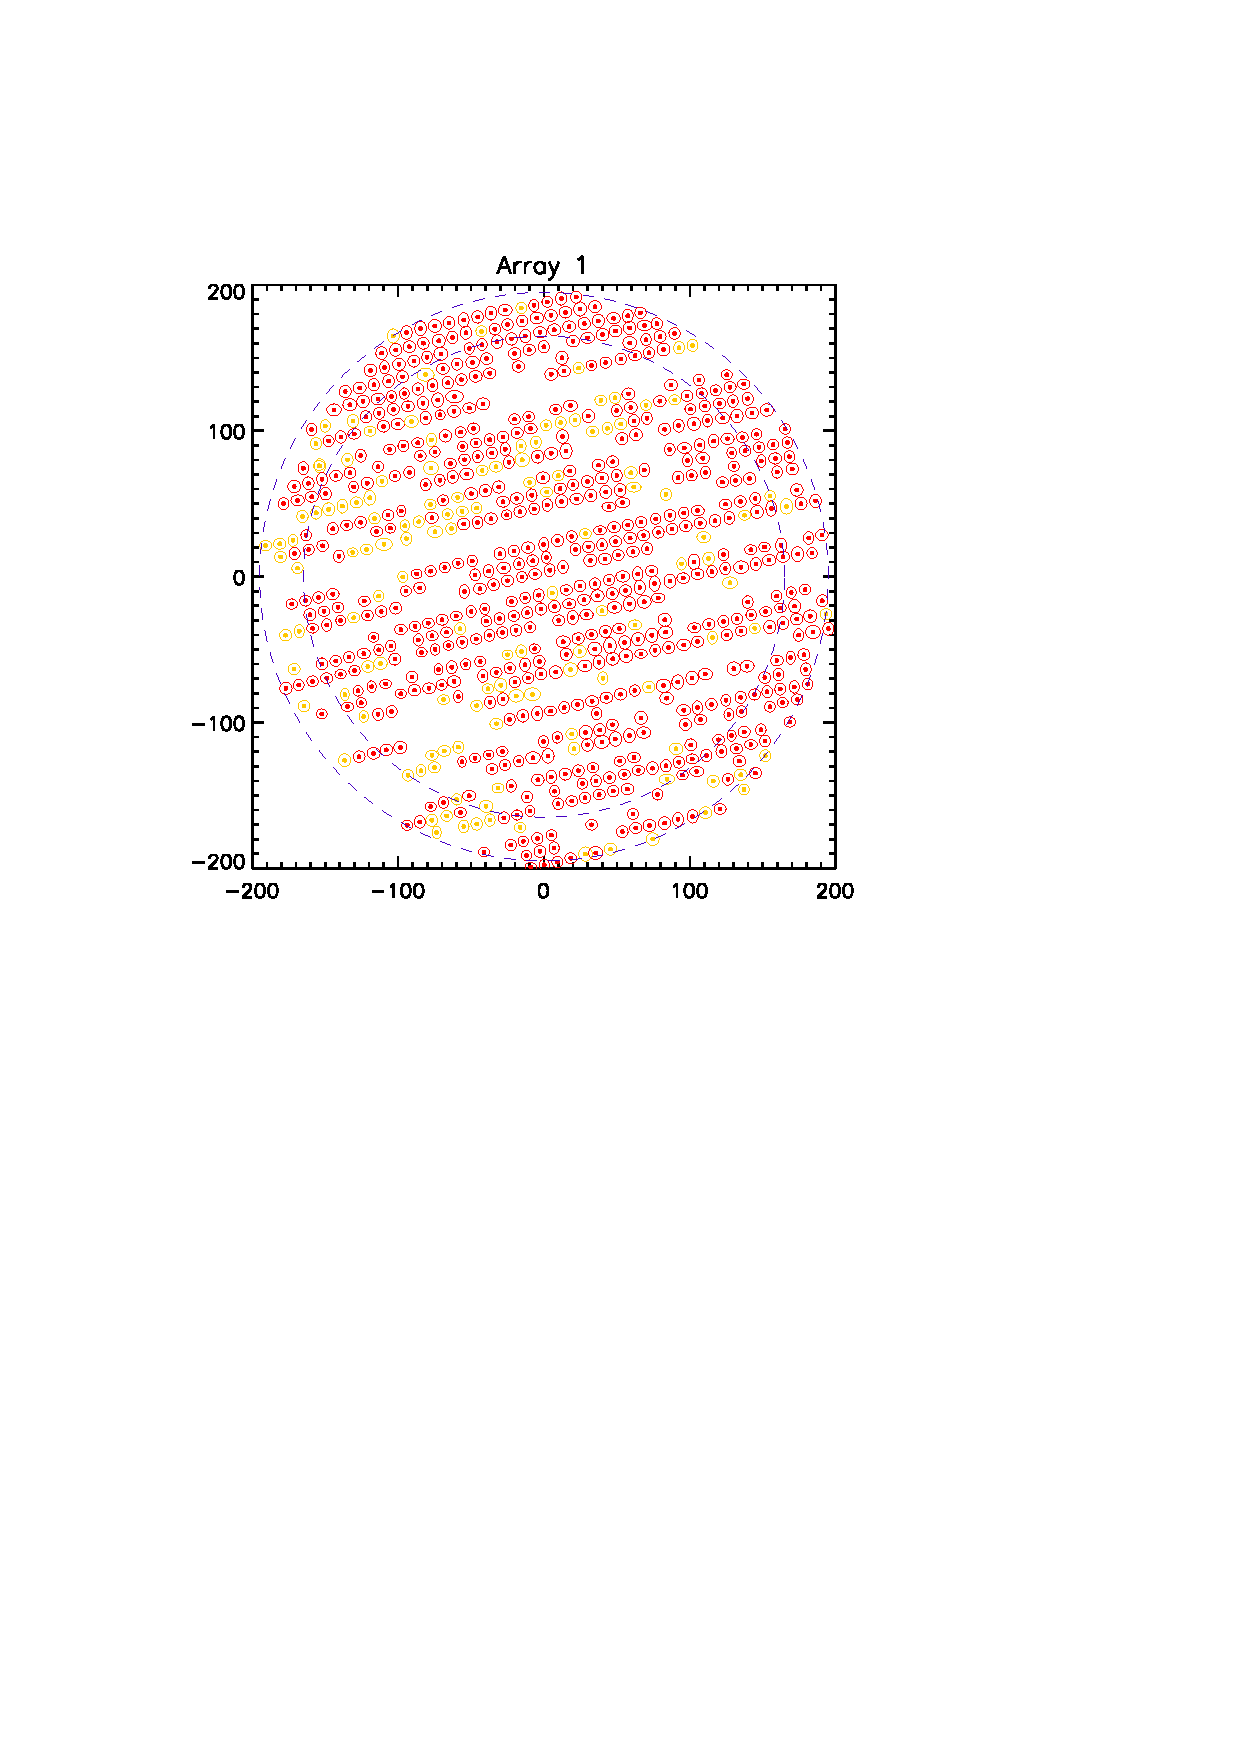
\includegraphics[trim=3cm 14cm 6cm 4cm, clip=true, width=0.32\linewidth]{Figures/NIKA2/A1_fwhm_color_count.pdf}
%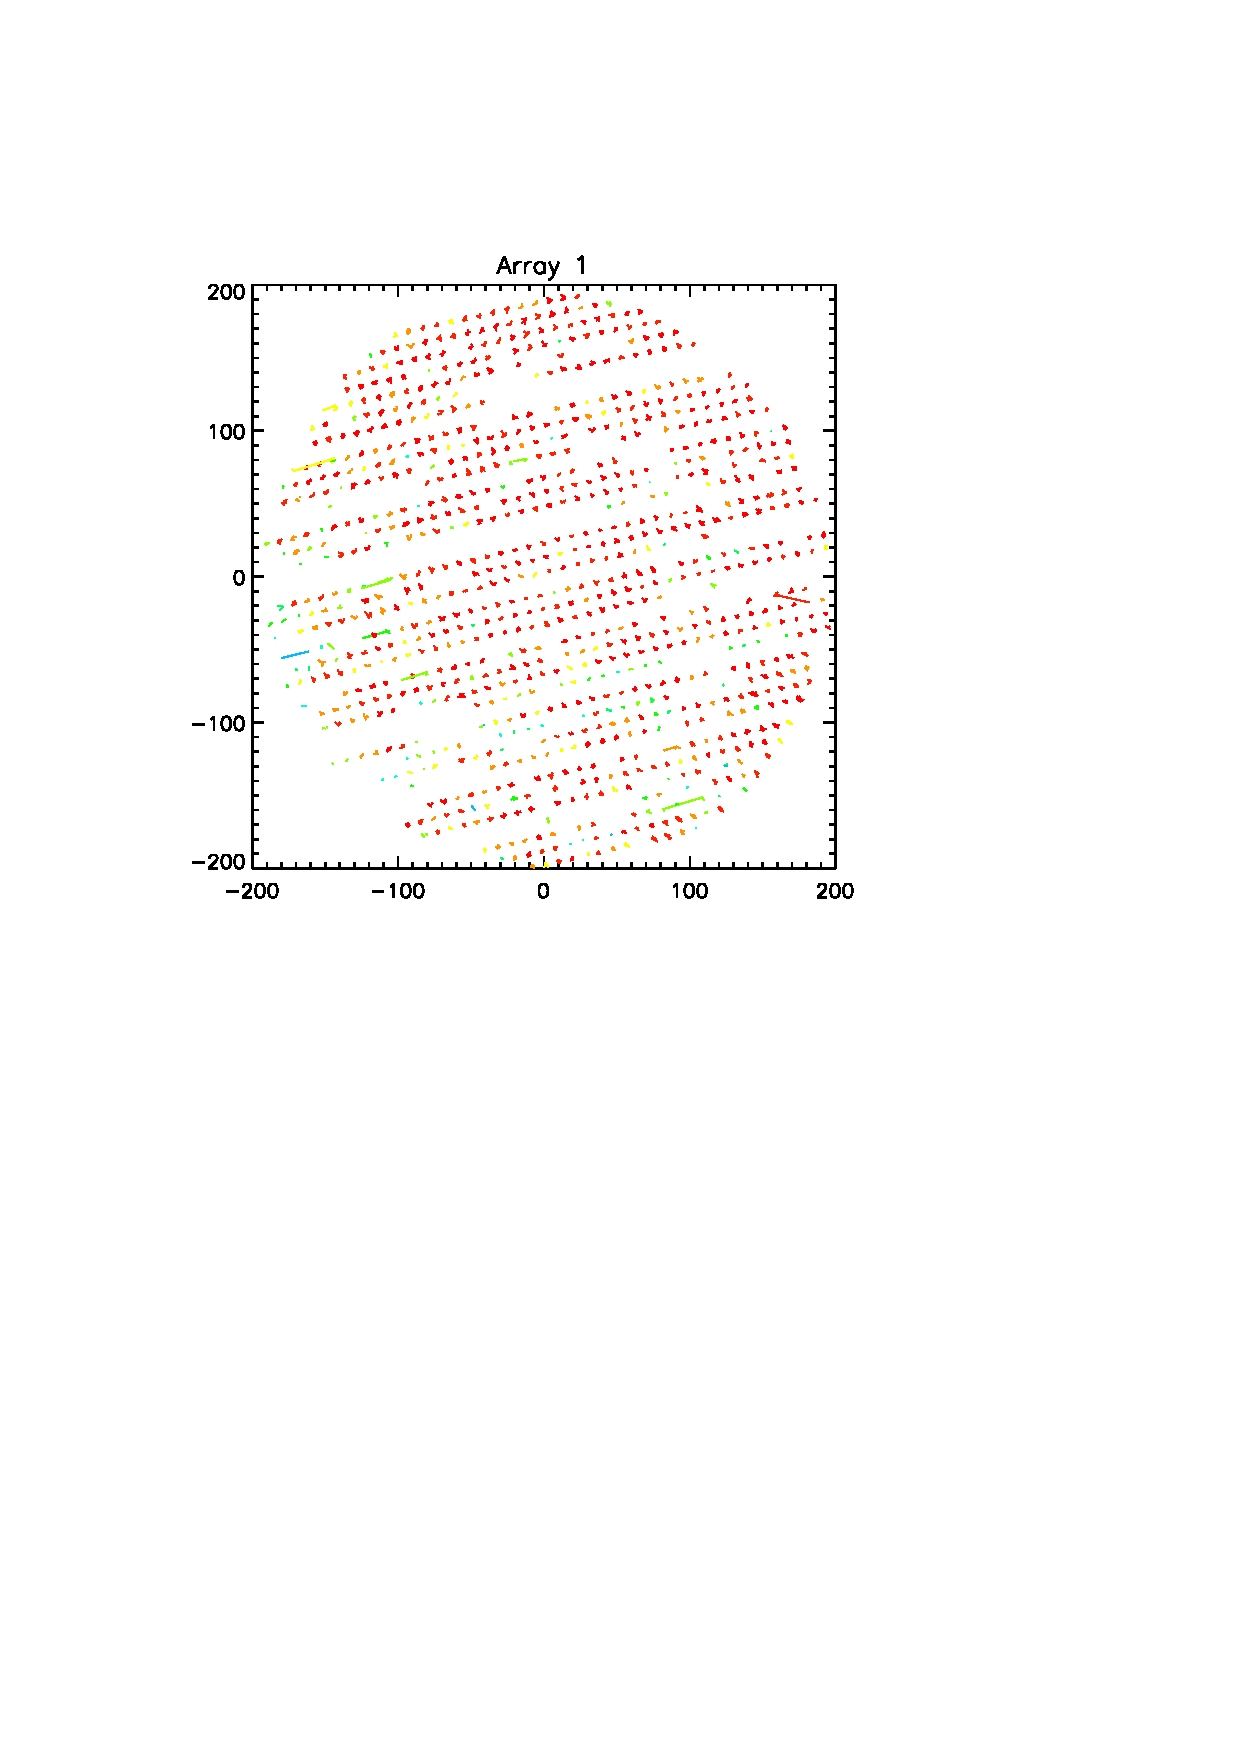
\includegraphics[trim=2cm 14cm 5cm 4cm, clip=true,width=0.45\linewidth]{Figures/A1_positions.pdf}
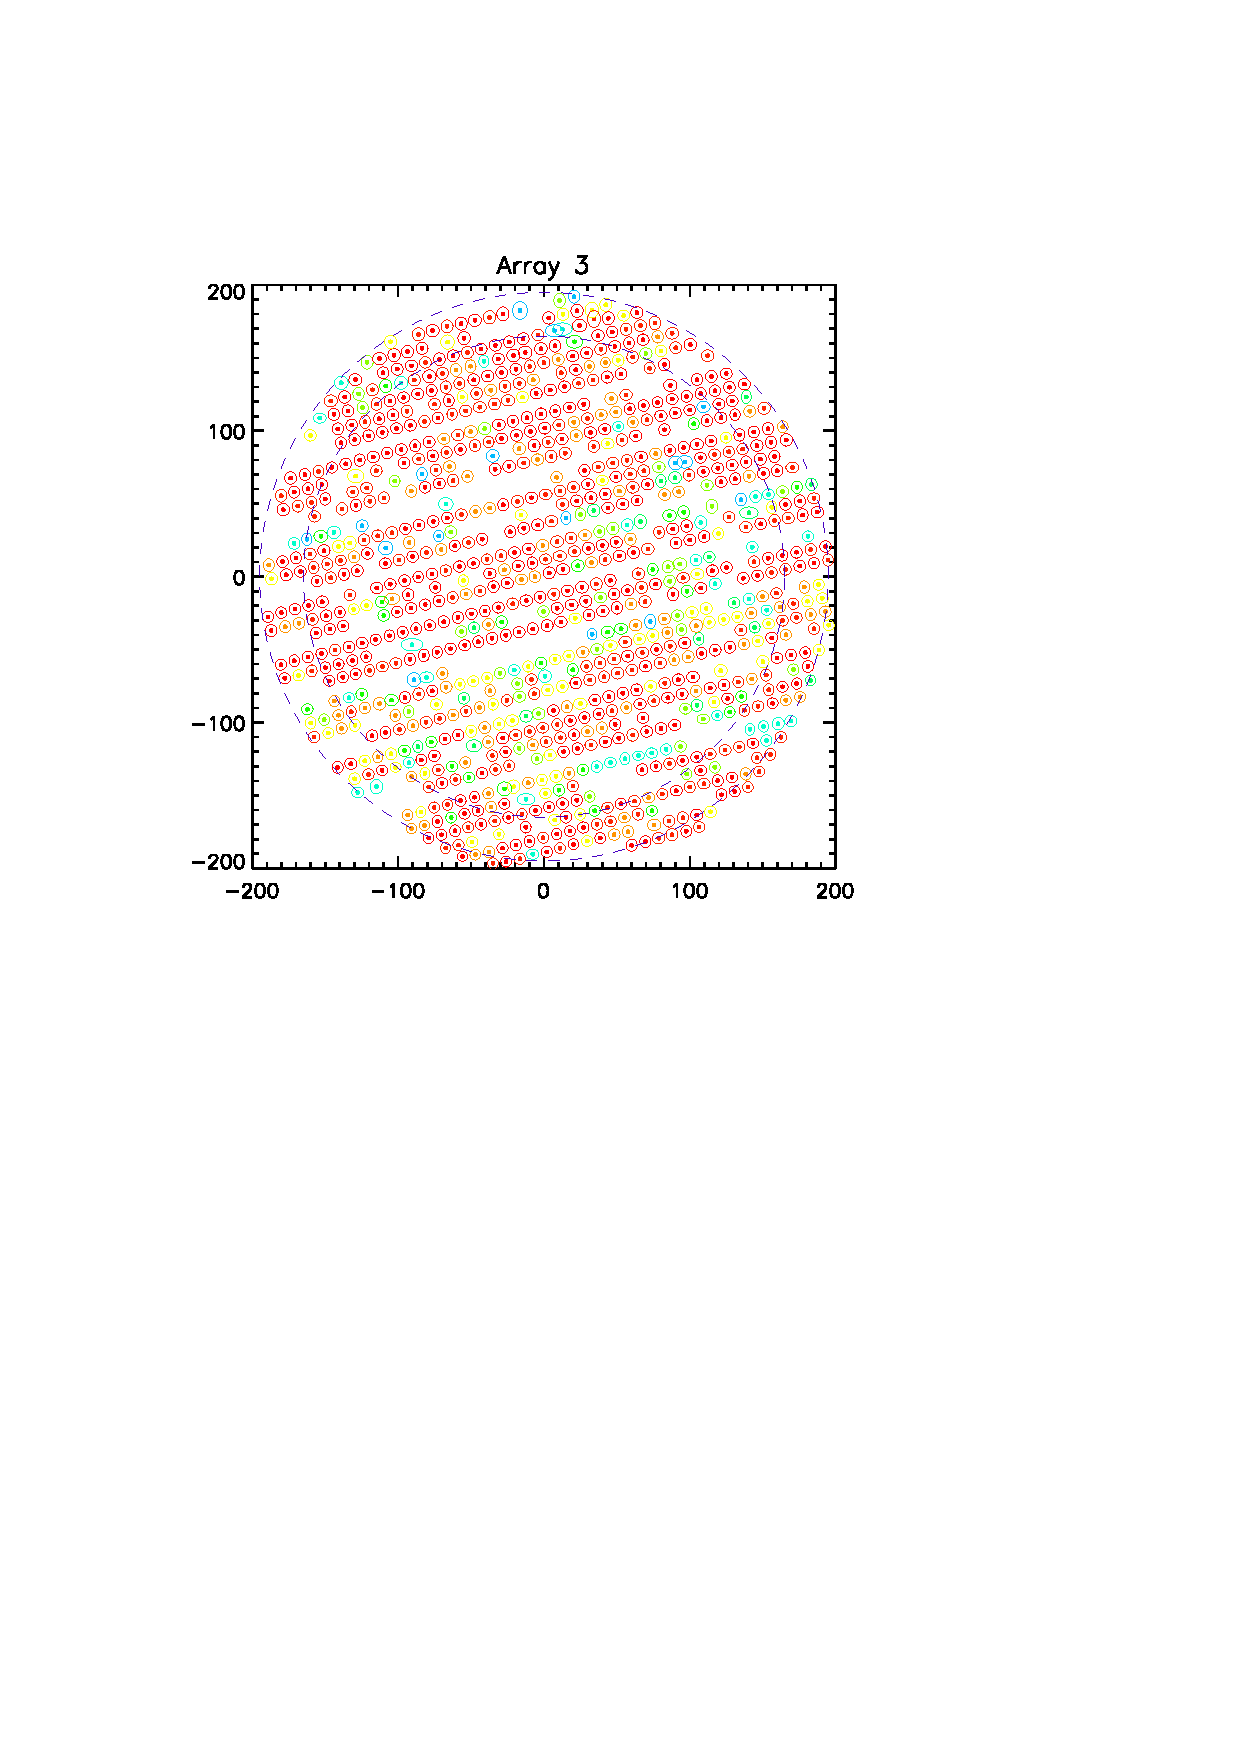
\includegraphics[trim=3cm 14cm 6cm 4cm, clip=true, width=0.32\linewidth]{Figures/NIKA2/A3_fwhm_color_count.pdf}
%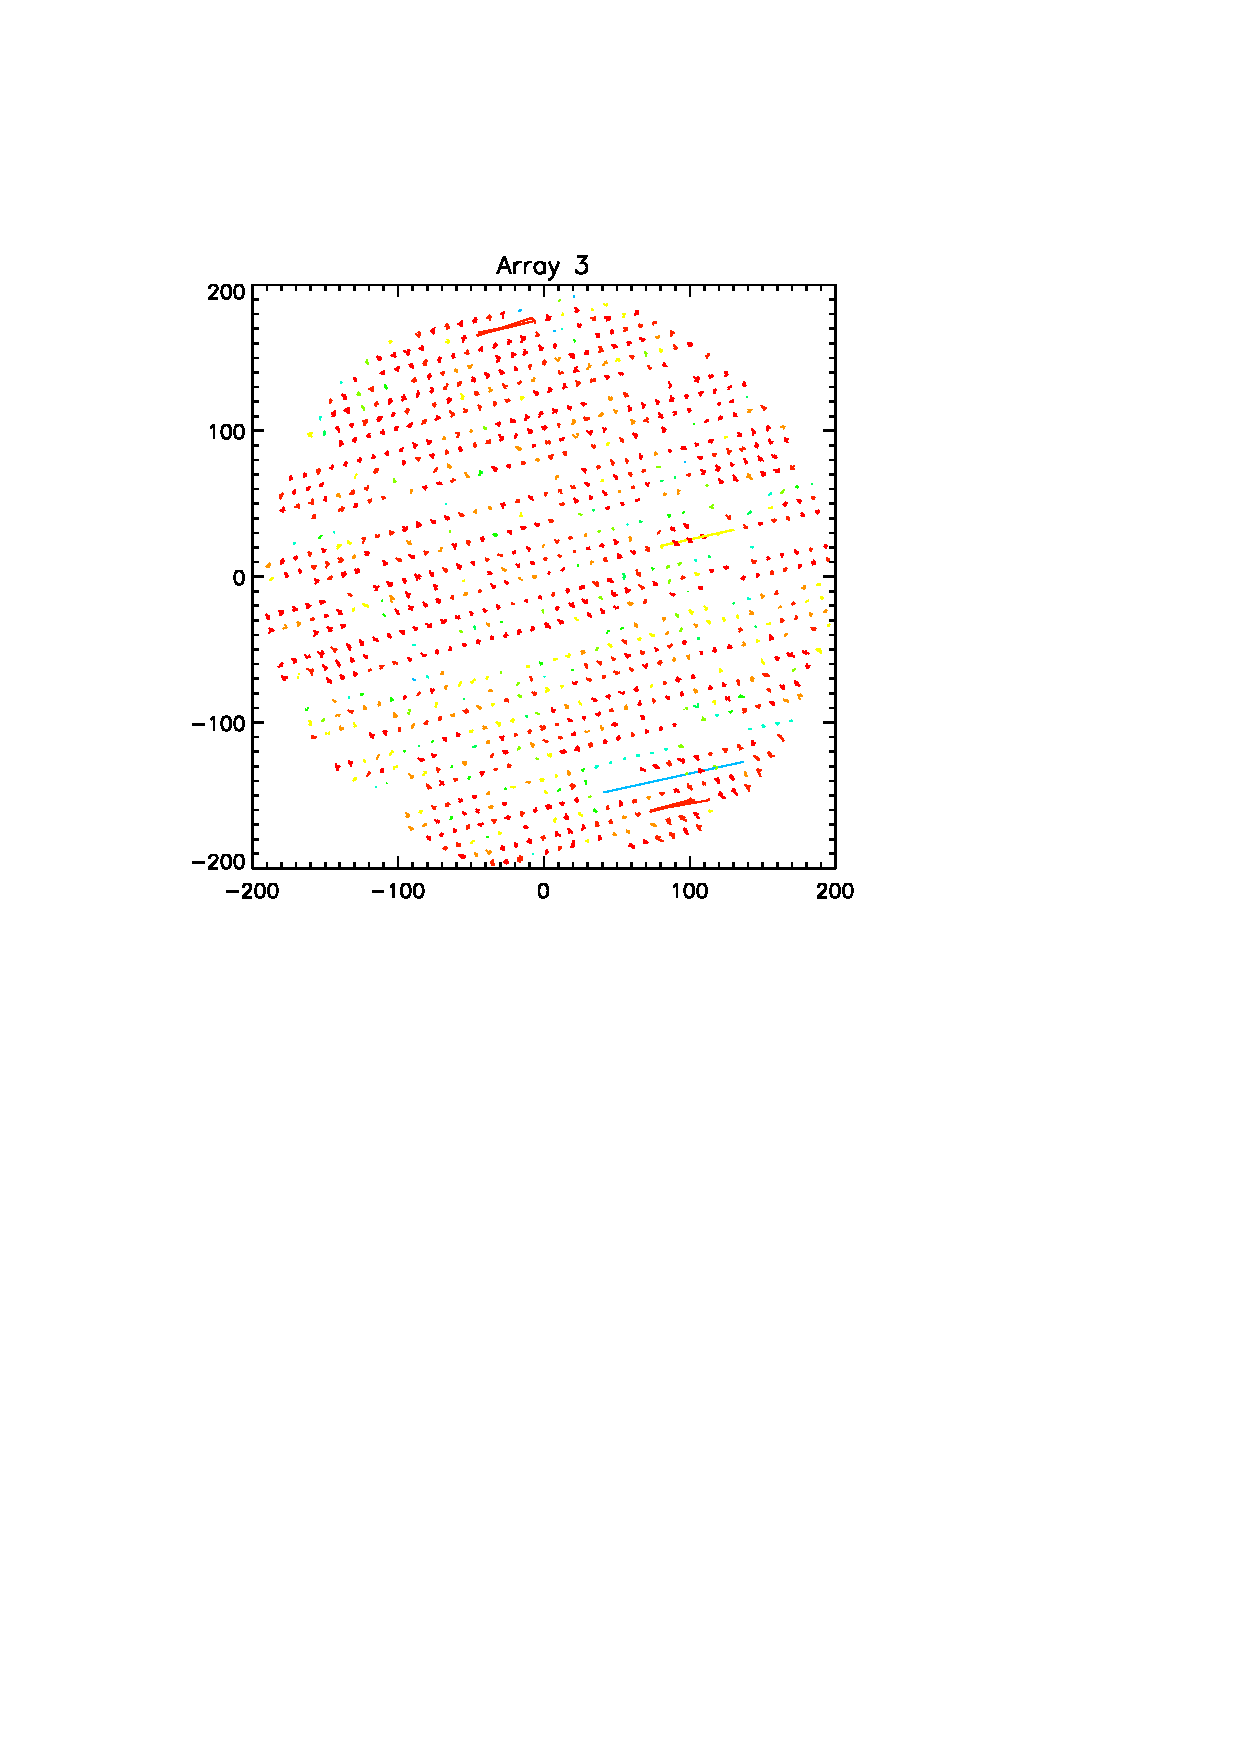
\includegraphics[trim=2cm 14cm 5cm 4cm, clip=true,width=0.45\linewidth]{Figures/A3_positions.pdf}
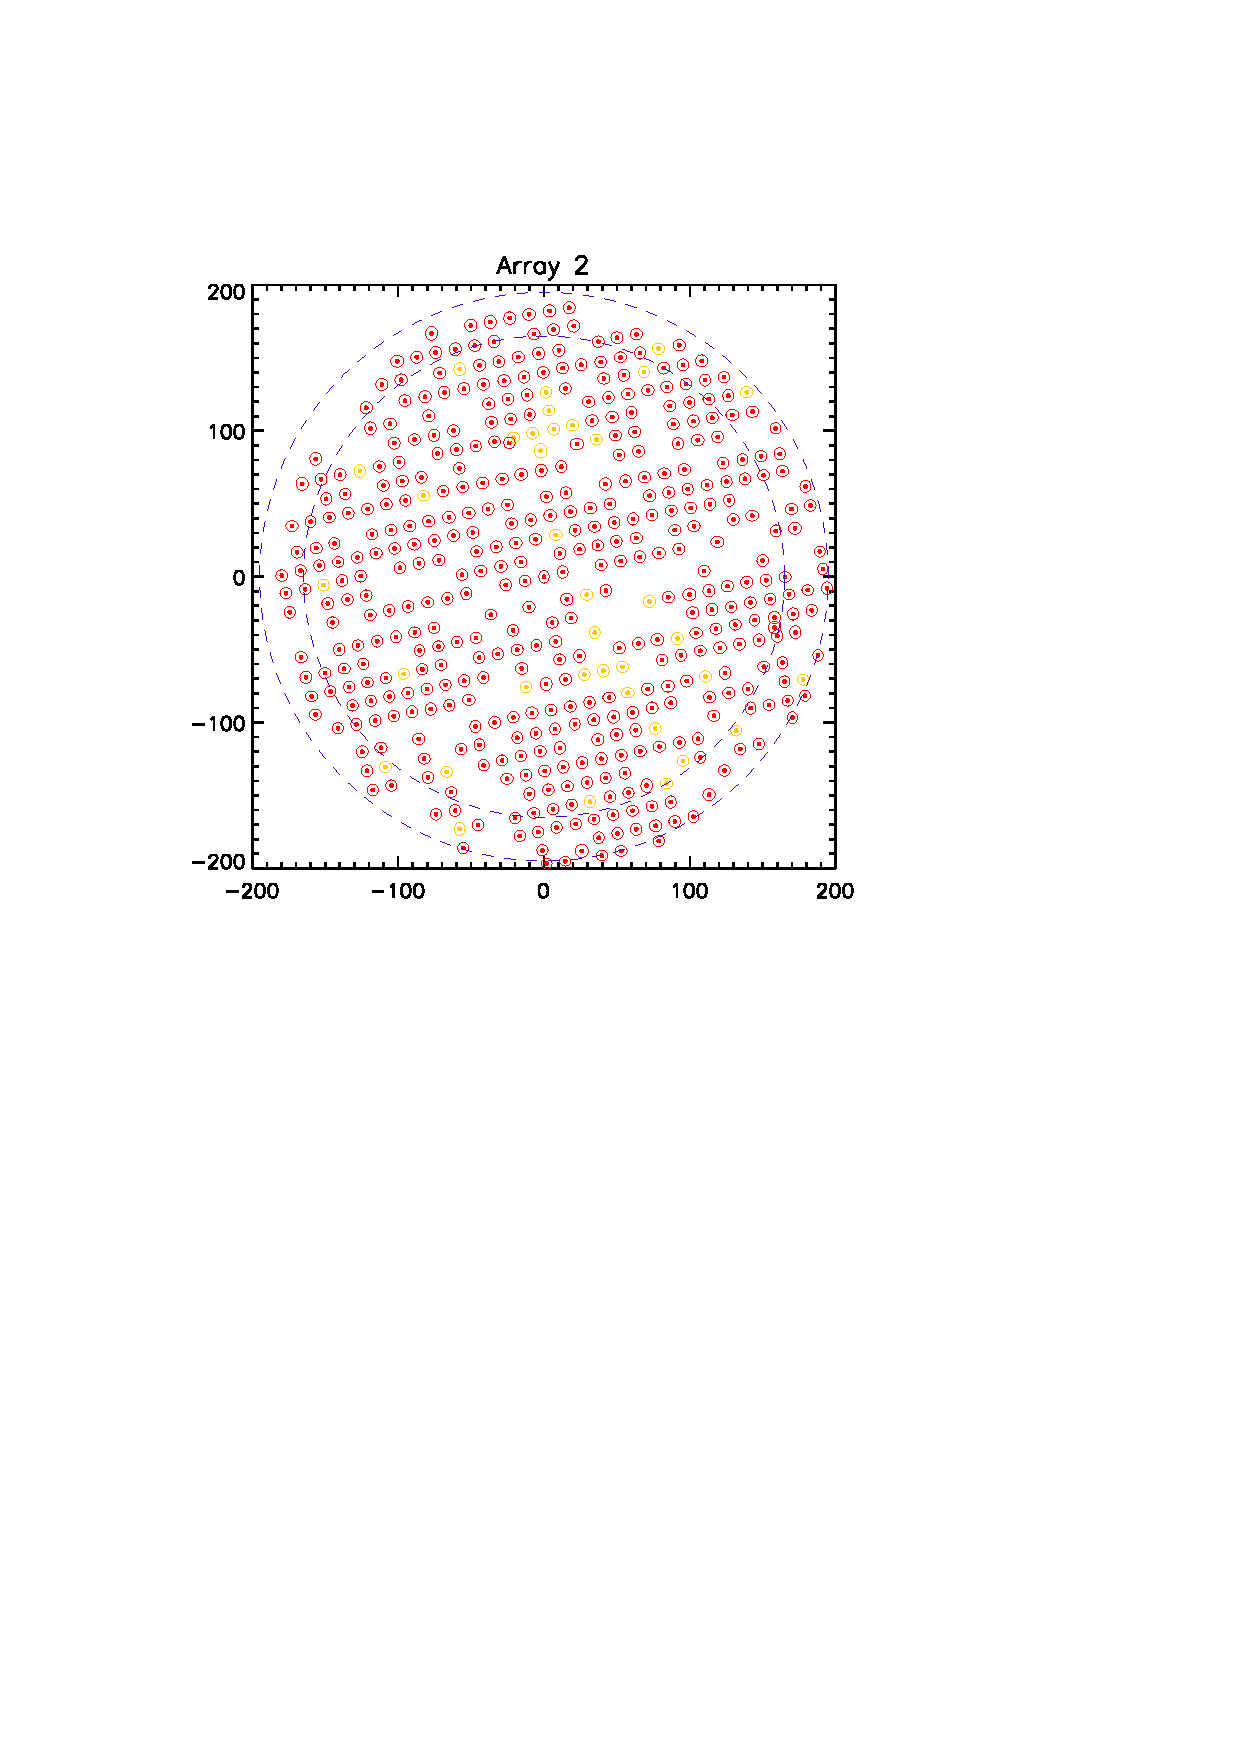
\includegraphics[trim=3cm 14cm 6cm 4cm, clip=true, width=0.32\linewidth]{Figures/NIKA2/A2_fwhm_color_count.pdf}
%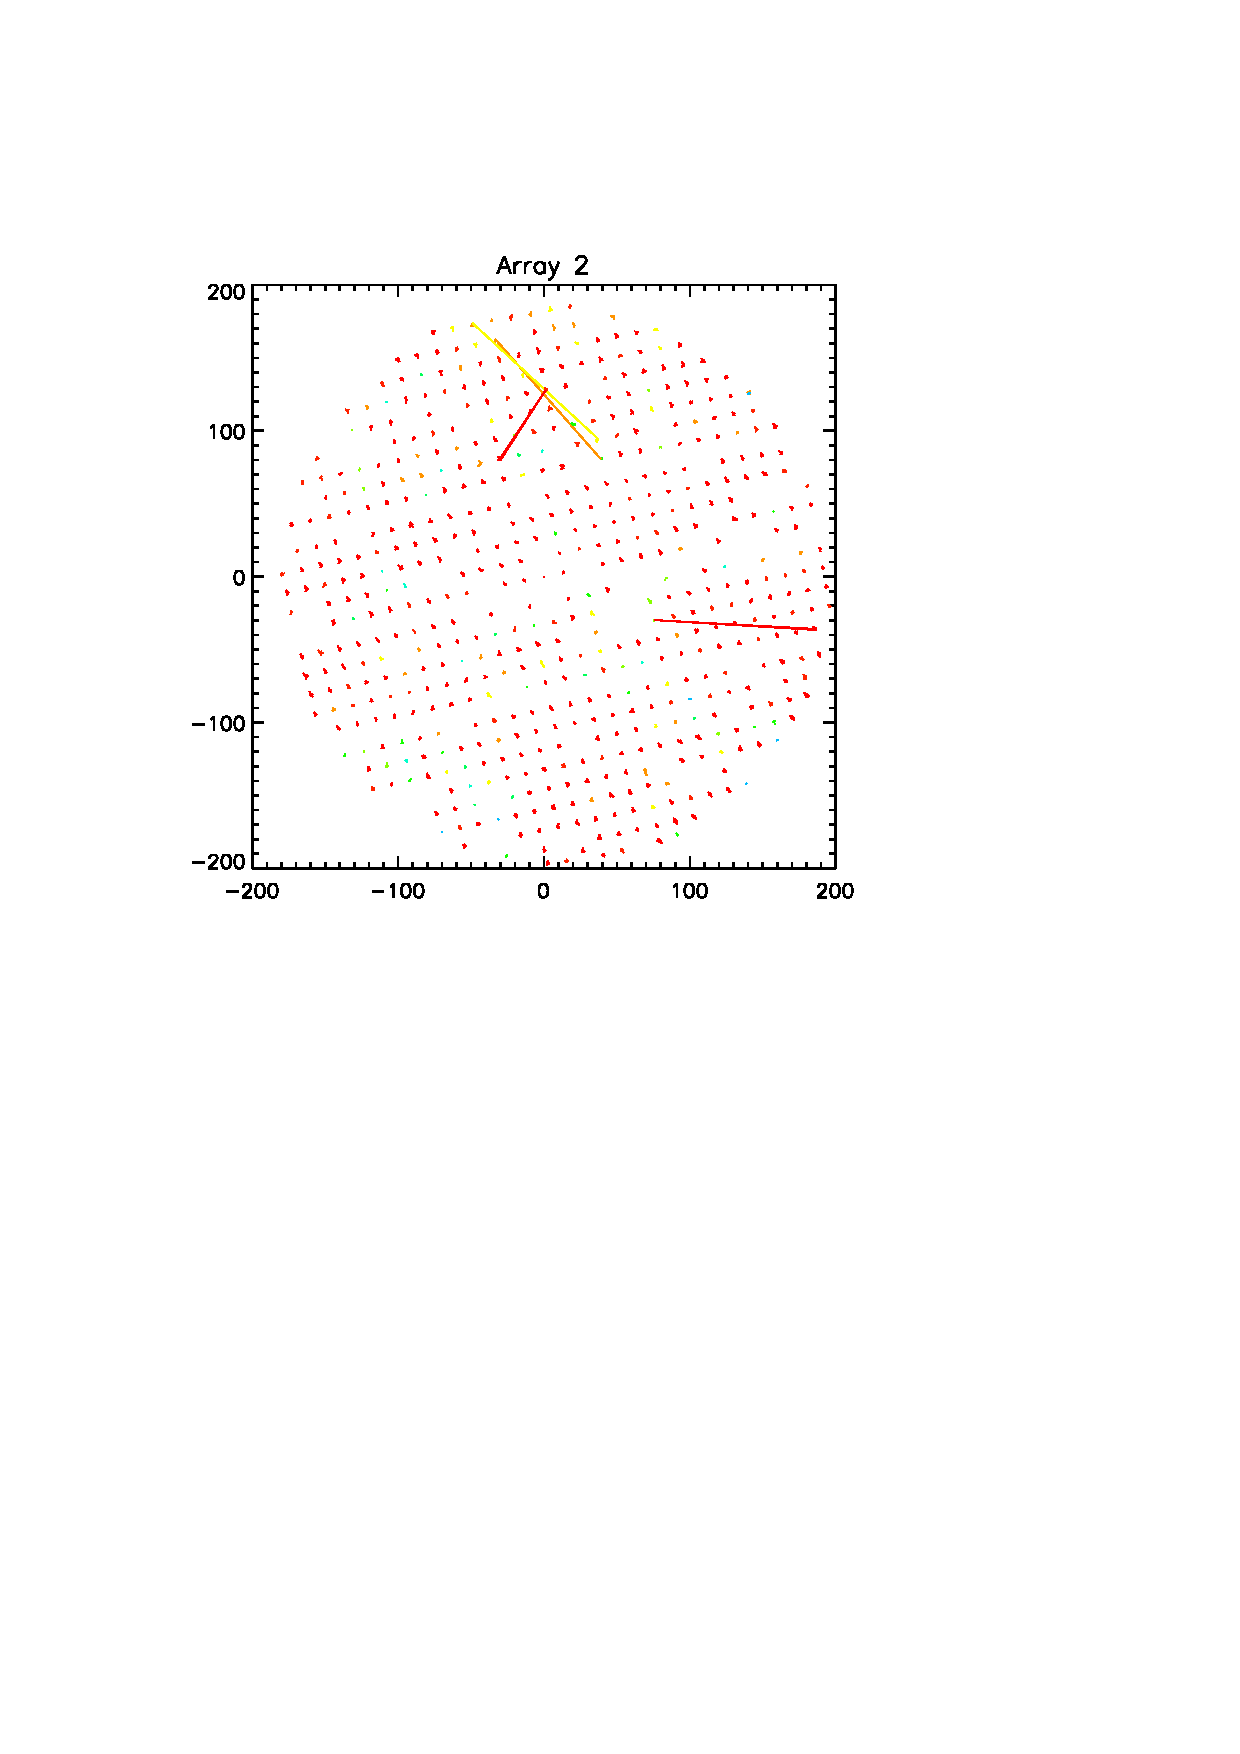
\includegraphics[trim=2cm 14cm 5cm 4cm, clip=true,width=0.45\linewidth]{Figures/A2_positions.pdf}
\caption[La sélection des KID]{Géométrie moyenne des matrices A1, A3
  et A2. Chacune des figures montre la position des détecteurs
  dans le plan focal, en secondes d'arc, ainsi que leur lobe modélisé par une
  gaussienne elliptique. Elles incluent les détecteurs qui ont été sélectionnés
  dans au moins deux analyses de {\tt beammaps}, correspondant à 952,
  961, and 553 KID pour A1, A3 et A2, respectivement.
  Les couleurs indiquent le nombre de fois qu'un KID a été
  sélectionné, depuis le bleu pour les KID sélectionnés dans deux
  analyses, jusqu'au rouge pour les KID sélectionnés dans les dix
  analyses (en passant par bleu ciel (3/10),
  cyan (4/10), céladon (5/10), vert (6/10), vert-jaune (7/10), jaune (8/10), orange (9/10)) 
  Les cercles en lignes interrompues correspondent à des disques de
  diamètres 5,5\,arcmin and 6,5\,arcmin.}
\label{fig:avg_fov_color}
\end{center}
\end{figure}

La sélection finale est obtenue par comptage du nombre
de fois qu'un KID a été sélectionné dans un ensemble de {\tt
  beammaps}. Le résultat de ce comptage est symbolisé par les couleurs
à la figure~\ref{fig:avg_fov_color} : depuis le bleu, indiquant les KID
sélectionnés dans deux analyses, jusqu'au rouge, pour les KID
sélectionnés dans les dix analyses. Nous définissons les KID
"valides'', c'est-à-dire à utiliser pour l'exploitation scientifique,
comme ceux qui ont été sélectionnés dans au moins 20\% des analyses de
{\tt beammaps} (2/10). Nous trouvons une fraction de KID valides de
84\% à 1\,mm et de 90\% à 2\,mm. Par ailleurs, l'ensemble du champ de
vue de 6,5' de diamètre, repéré par le cercle externe à la
figure~\ref{fig:avg_fov_color}, est bien couvert par les détecteurs
pour les trois matrices. 




%----------------------------------------------------------------------------------------
%
%   Lobe
%
%----------------------------------------------------------------------------------------
\section{Le lobe}
\label{se:beam}

Le lobe de NIKA2 résulte de l'illumination par les détecteurs de l'ensemble
du système optique jusqu'au miroir primaire du télescope. Le lobe
total présente une structure complexe, incluant un lobe principal, des
lobes d'erreurs provenant de la déformation d'ensemble du miroir
primaire, et des lobes lointains résultant de la diffraction par
différentes structures composant le système optique. Nous en donnons
une description qualitative à la Sect.~\ref{se:fullbeam}, puis nous
estimons les paramètres du lobe déterminant les performances de NIKA2
à la Sect.~\ref{se:mainbeam} : la largeur à mi-hauteur (FWHM) du lobe
principal, définissant la résolution angulaire de l'instrument, et
l'efficacité du lobe principal, influant sa sensibilité. Finalement,
nous mesurons les varations temporelles du lobe principal à la
Sect.~\ref{se:fwhm_variations}.


\subsection{La structure du lobe total}
\label{se:fullbeam}

La structure du lobe total est mise en évidence en combinant plusieurs
{\tt beammaps} vers des sources compactes brillantes.
%%
\begin{figure}[!thbp]
\begin{center}
  \includegraphics[trim=0.5cm 0.5cm 1cm 0cm, clip=true, width=\linewidth]{Figures/NIKA2/Lobe_map_Combo_v2_dB_2.pdf}
\caption[Noticeable features of NIKA2 beam pattern.]{Cartographie du
  lobe de la combinaison des matrices à 1\,mm (A1$\&$3) and de la
  matrice à 2\,mm (A2) en décibels. Ces cartes sont construites à
  partir d'une combinaison de {\tt beammaps} vers des sources
  ponctuelles brillantes; elles sont en coordonnées horizontales et
  couvrent une zone du ciel de $10'$ de coté. En plus du lobe pricipal
  et des premiers lobes d'erreur et lobes lointains au centre, elles
  présentent plusieurs structures notables (comme l'anneau de
  diffraction à 1\,mm, les figures de diffraction par les pieds
  supportants le miroir secondaire à 2\,mm) qui sont commentées dans le
  texte.}
\label{fig:features}
\end{center}
\end{figure}
%%
\`A la figure~\ref{fig:features}, nous présentons une cartographie du lobe
total incluant quatre {\tt beammaps} vers Uranus, Neptune et le quasar
3C84. Des cartes sont produites à partir de chaque {\tt beammap} en
utilisant le \emph{pipeline} d'analyse décrit à la
Sect.~\ref{se:pipeline}, puis elles sont normalisées et recentrées avant d'être
co-additionnées. Les cartes finales mettent au jour la structure du
lobe sur quelques minutes d'arc, les plus grandes échelles angulaires
étant filtrées par la méthode d'analyse. Elles révèlent une structure
complexe incluant 1) le lobe principal (point central) et les premiers
lobe d'erreur et lobes lointains du télescope, visibles au centre à un
niveau jusqu'à -20 décibel, 2) un anneau de rayon environ 110'',
visible à un niveau bien plus faible (-30\,dB) à 1\,mm, et qui
tirerait son origine de la diffraction par les jointures des panneaux
composant le miroir primaire~\citep{Greve2010}, 3) deux diagonales,
visibles également vers -30\,dB sur la carte à 2\,mm, créées par la
diffraction par la structure (quadrupode) supportant le miroir
secondaire, 4) d'autres petites structures à des niveaux situés en
deça de -20\,dB, d'origine incertaines, ayant très peu d'impact sur
les observations.


Une autre manière de caractériser le lobe total, permettant de mesurer
les contributions relatives des principales structures le composant,
consiste à mesurer son profil radial. Celui-ci est obtenu en moyennant
les pixels de la carte du lobe dans des anneaux concentriques autour
du lobe principal. \`A la figure~\ref{fig:beam_prof}, nous traçons les
profils du lobe mesurés à partir de 18 {\tt beammaps}. Ce jeu de {\tt
  beammaps} nous permet de tester la stabilité du profil du lobe sous
différentes conditions d'observation (densité de flux de la source,
conditions atmosphériques, élévation, optimisation du focus). La
dispersion des profils par rapport au profil médian est de $5\%$ à
1\,mm et $2\%$ à 2\,mm, indiquant une bonne stabilité. Par ailleurs,
le profil du lobe est bien mesuré jusqu'à un rayon d'environ
180''.

\begin{figure}[!thbp]
  \centering
   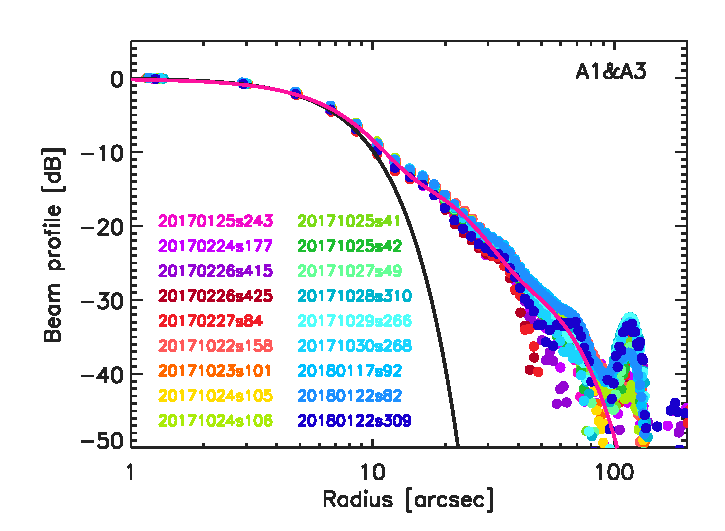
\includegraphics[clip, width=0.45\linewidth]{Figures/NIKA2/plot_profiles_dB_1mm.pdf}
   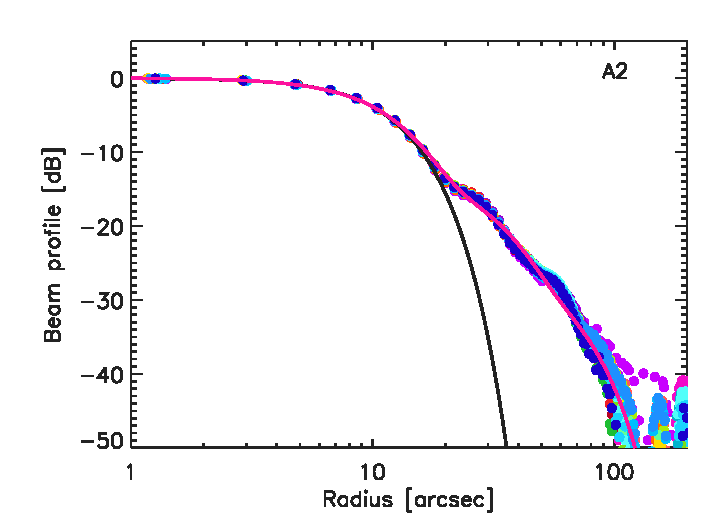
\includegraphics[clip, width=0.45\linewidth]{Figures/NIKA2/plot_profiles_dB_a2.pdf}
   \caption[Stability of the beam profile]{Profiles radiaux des lobes
     à 1\,mm (à gauche) et 2\,mm (à droite) tracés en décibels en
     fonction de la distance radiale au centre du lobe. Les points
     correspondent à la mesure du profile du lobe pour une série de 18
     {\tt beammaps} vers des sources compactes brillantes observés
     lors des campagnes de référence. Ils sont repérés par
     l'identifiant du scan de {\tt beammaps}. La courbe rose montre le
     modèle 3G calculé à partir de la médiane des meilleurs ajustement
     sur chacun des profiles. La courbe noire représente le meilleur
     ajustement d'une gaussienne au lobe principal.}
  \label{fig:beam_prof}
\end{figure}

Pour estimer les contributions relatives des premiers lobes
d'erreur et lobes lointains, nous modélisons le profil par une
combinaison linéaire de trois gaussiennes (3G). Un profil 3G est
ajusté à chacun des 18 profils mesurés et la médiane des meilleurs
ajustements est tracée à la figure~\ref{fig:beam_prof}. Nous mesurons
la contribution du premier lobe d'erreur par rapport au lobe total à
-11\,dB à 1\,mm et à -13\,dB à 2\,mm. Le lobe principal, modélisé par
une gaussienne, est tracé en noir à la figure~\ref{fig:beam_prof}. 


\subsection{Le lobe principal}
\label{se:mainbeam}

\subsubsection{La FWHM}

Le lobe principal est bien modélisé par une gaussienne. L'ajustement
de cette gaussienne aux cartes ou aux profils du lobe total doit
prendre en compte la contribution des lobes d'erreur et lobes
lointains. Pour cela, trois méthodes ont été développées. La première
repose sur l'ajustement d'un profil 3G (Sect.~\ref{se:fullbeam}) : la
première gaussienne correspondant au lobe principal tandis que les
deux autres capturent les autres contributions au lobe total. Les deux
autres méthodes consistent à ajuster une unique gaussienne au lobe
total, en masquant les distances radiales pour lesquelles la
contribution des lobes d'erreur et lointains est significative. Ces
méthodes sont détaillées dans~\citet{Perotto2019}. Testées sur
plusieurs jeux de données, variant de part la stratégie de scans ({\tt
OTF}-scans ou {\tt beammaps}), les sources observées et les campagnes
d'observation, ces méthodes donnent des résultats cohérents et
compatibles, indiquant la robustesse de la mesure de la FWHM du lobe
principal.


Nous testons en particulier, la stabilité des FWHM mesurées pour des
conditions atmosphériques variables. Pour cela, nous avons constitué
un jeu de données comprenant environ 150 scans OTF vers des sources
compactes dont le flux excède 1\,Jy dans les deux bandes de fréquence,
sélectionnés en appliquant les critères définis à la
Sect.~\ref{se:scan_selection} aux trois campagnes d'observation de
référence. \`A la figure~\ref{fig:fwhm_map_atmtrans}, les mesures de
la FWHM effectuées à partir de ce jeu de données sont tracées en
fonction de la transmission atmosphérique, modélisée par
$\exp{(-\taunu\,x)}$. Le code de couleur indique la campagne
d'observation lors de laquelle a été acquis le scan. Nous concluons
que les mesures de la FWHM sont en accord pour les trois campagnes de
référence, et n'observons par d'effet systématique significatif
dépendant de la transmission atmosphérique.
%
\begin{figure}[!thbp]
\begin{center}
  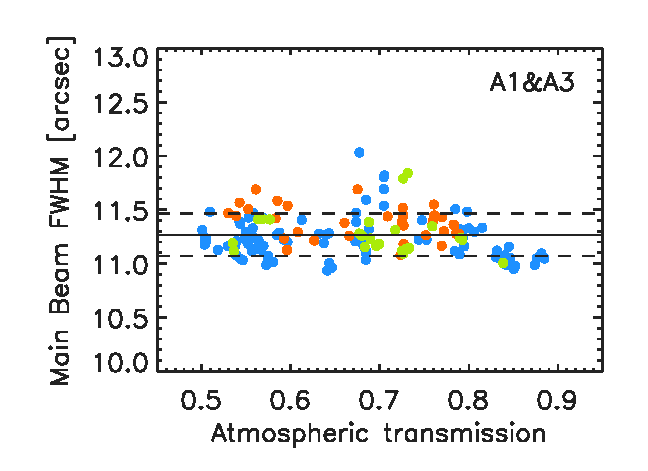
\includegraphics[clip, width=0.4\textwidth]{Figures/NIKA2/plot_FWHM_vs_atmtrans_mb_radius_binning2_1mm.pdf}
  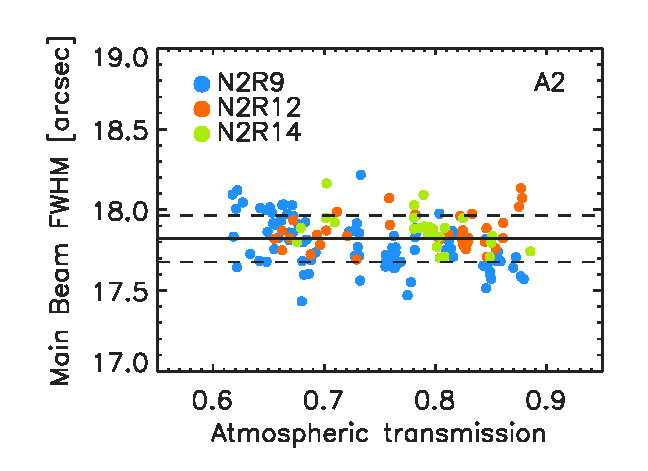
\includegraphics[clip, width=0.4\textwidth]{Figures/NIKA2/plot_FWHM_vs_atmtrans_mb_radius_binning2_a2.pdf}
  \caption[Main Beam FWHM]{Estimations de la largeur à mi-hauteur
    (FWHM) du lobe principal modélisé par une gaussienne, pour la bande à 1\,mm
    (à gauche) et à 2\,mm (à droite). Les FWHM sont mesurées à partir
    d'une série d'observations de sources compactes de flux $>1\,$Jy
    effectuées lors des trois campagnes de référence (N2R9, N2R12,
    N2R14); elles sont tracées en fonction de la transmission de
    l'atmosphère au moment de l'observation, qui dépend de l'opacité
    de l'atmosphère le long de la ligne de visée, $\taunu \, x$,
    suivant $\exp{(-\taunu \, x)}$. }
\label{fig:fwhm_map_atmtrans}
\end{center}
\end{figure}
%
En combinant les résultats des tests effectués avec différentes
méthodes d'estimation et différent jeux de données, nous obtenons une
mesure robuste de la FWHM et de son incertitude. Le lobe principal est
caractérisé par une FWHM de $11,1'' \pm 0,2''$ à 260\,GHz et de
$17,6'' \pm 0,1''$ à 150\,GHz. Ces performances sont meilleures que
les spécifications définies dans MoU. 


\subsubsection{L'efficacité}

L'efficacité du lobe principal est définie comme l'angle solide
soutendu par le lobe principal rapporté à l'angle solide du lobe
total. L'angle solide du lobe principal (\emph{main beam}) se calcule
directement à partir de la FWHM suivant $\Omega_{\rm{mb}} = 2\pi\,
(8\ln{2} \, \rm{FWHM}^2)$. L'angle solide du lobe
total jusqu'à une distance radiale maximale $r_{\rm{max}}$ est évalué suivant
\begin{equation}
  \Omega_{r_{\rm{max}}}(\nu) = \int_0^{r_{max}} B_{\nu}(r) \,  2 \pi r dr
  \label{eq:omega_rmax}
\end{equation}
à partir du profil normalisé du lobe total $B_{\nu}(r)$ pour la
matrice $\nu$. Nous le mesurons dans les cartes produites à partir de
{\tt beammaps} vers une source ponctuelle jusqu'à
$r_{\rm{max}}=180''$. Cette limite est imposée à la fois par la
stratégie de balayage, qui détermine l'homogénéité et le niveau de
bruit dans les cartes, et par le filtrage des grandes échelles
angulaires induit par le \emph{pipeline} d'analyse
(Sect.~\ref{se:pipeline}). \`A partir des mesures du profil du lobe
total et de la FWHM du lobe principal, nous estimons une efficacité de
$55 \pm 3\%$ à 260\,GHz et de $77 \pm 2\%$ à 150\,GHz.

Des études dédiées au lobe du télescope de 30-m ont qu'une
fraction significative du lobe se situe à des distances radiales au-delà
de 180''~\citep{Greve1998, Kramer2013}. Dans \citet{Kramer2013}, le
profil du lobe total a été mesuré à partir d'observations des limbes
de la Lune et modélisé par un lobe principal et trois lobes d'erreurs
gaussiens. Cette étude évalue également les contributions aux grandes échelles
angulaires à l'efficacité, issues du \emph{spillover}
(lumière parasite issue de l'atmosphère et du sol) et de Ruze (effet
des écarts de la surface du miroir primaire à la forme parabolique), à
partir d'observations de type {\tt skydip} effectuées avec le
\emph{Eight Mixer Receiver} (EMIR, \citet{Carter2012}),
l'instrument hétérodyne installé au télescope de 30-m. En nous fondant
sur ces résultats, nous évaluons l'angle solide du lobe total comme
\begin{equation}
  \Omega_{\rm{tot}} = \Omega_{180} + \Omega_{>180}^{\rm{mb+eb}} +
  \Omega^{\rm{frss}},
  \label{eq:omega_tot}
\end{equation}
où $\Omega_{180}$ est la mesure de l'angle solide du lobe total
jusqu'à 180'' estimée en utilisant Eq.~\ref{eq:omega_rmax},
$\Omega_{>180}^{\rm{mb+eb}}$ est la contribution des distances
radiales $>180''$ à l'angle solide issue du lobe principal (mb) et des
lobes d'erreur (eb) modélisés suivant~\citet{Kramer2013}, et
$\Omega^{\rm{frss}}$ représente les contributions du \emph{spillover}
et de la dispersion de Ruze. Ces différents termes sont évalués
dans~\citet{Perotto2019}. Chacun représente entre 7 et 15\% de l'angle
solide total. Cette caractérisation de l'angle solide total
est nécessaire à l'étude des sources diffuses ou aux mesures de flux
par photométrie d'ouverture, comme discuté plus loin, à la
Sect.~\ref{se:calibration}.


\subsection{Variation journalière}
\label{se:fwhm_variations}

\`A partir de tests de stabilité du lobe principal, nous
avons mis au jour une variation journalière de la FWHM. Cette
variation consiste en une lente augmentation de la FWHM, débutant
après le lever du Soleil et devenant significative dans l'après-midi,
puis un retour vers la valeur nominale (nocturne) après le coucher du
Soleil. Cet effet est présenté à la
figure~\ref{fig:beam_monitoring_otf} rassemblant les mesures de la
FWHM effectuées à partir d'une série de scans OTF vers des sources
compactes brillantes, et tracées en fonction de l'heure
d'observation. Une même évolution globale de la FWHM durant la journée
est observée lors des trois campagnes de référence. Cette variation
journalière est indépendante du flux de la source, puisqu'elle reste
la même aussi bien à partir des scans vers les planètes géantes Uranus
et Neptune que vers d'autres sources compactes moins brillantes. Par
ailleurs, d'importantes variations sont observées autour de la
tendance globale.
%
\begin{figure}[ht!]
  \begin{center}
    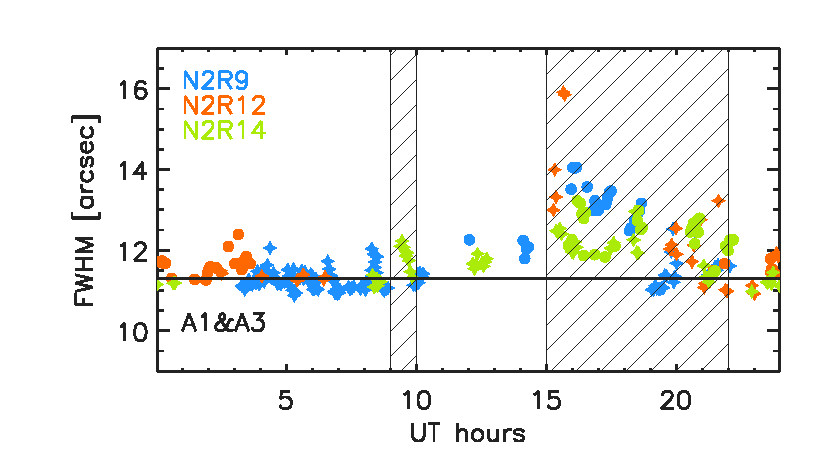
\includegraphics[clip=true, trim={0.9cm, 0.5cm, 0.5cm, 0.5cm}, width=0.4725\textwidth]{Figures/NIKA2/Beam_monitoring_with_otfs_vs_ut_1mm.pdf}
    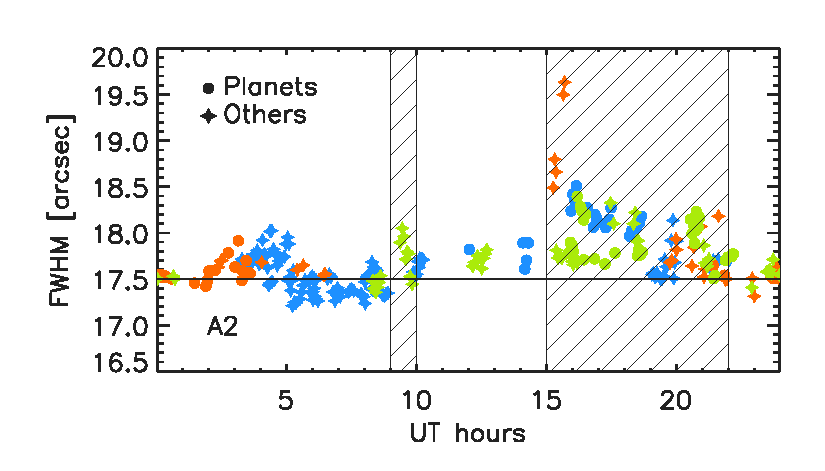
\includegraphics[clip=true, trim={0.5cm, 0.5cm, 0.5cm, 0.5cm}, width=0.4875\textwidth]{Figures/NIKA2/Beam_monitoring_with_otfs_vs_ut_a2.pdf}
    \caption[Beam size monitoring using OTF scans]{Suivi des
      variations journalières de la taille apparente du lobe. La
      largeur à mi-hauteur (FWHM) du lobe, modélisé par une gaussienne
      elliptique, est tracée pour la bande à 1\,mm (à gauche) et à
      2\,mm (à droite) en fonction du moment d'observation exprimé en
      heures UTC. Les mesures sont effectuées à partir de scans vers
      les planètes géantes (points) et vers d'autres sources
      compactes de flux $>1\,\rm{Jy}$ (étoiles) observés durant les
      trois campagnes de référence. Les zones hachurées correspondent
      aux périodes d'observation exclues par la sélection
      \emph{baseline} des scans, décrite à la Sect.~\ref{se:scan_selection}.} 
\label{fig:beam_monitoring_otf}
  \end{center}
\end{figure}

Cette variation journalière résulte probablement de la combinaison de
deux phénomènes liés à la température extérieure. Tout d'abord, le
chauffage inhomogène du miroir primaire du télescope, par exemple sous
l'effet de l'illumination partielle par la lumière solaire, entraîne
des déformations d'ensemble, qui à leur tour, le défocalisent
légèrement. L'impact de cet effet est réduit grâce au système de
thermalisation qui équipe le miroir primaire (voir
Sect.~\ref{se:observations}), mais dans les cas de forts gradients de
température d'un bout à l'autre des 30\,m de diamètre, un effet
résiduel peut apparaître. Ces variations journalières sont connues au
télescope de 30-m : elles impactent également les observations de
l'instrument EMIR et avaient été mises en évidence avec
MAMBO-2~\citep{Kreysa1999}, l'instrument ayant précédé l'intallation
de NIKA et NIKA2. Cependant, l'amplitude de l'effet est certainement
en augmentation depuis quelques années, avec la progressive
dégradation de la peinture blanche recouvrant le miroir primaire.

Le deuxième effet qui participe de la variation journalière du lobe,
est la refraction anormale de l'atmosphère. Ce phénomène, qui a été
décrit pour le télescope de 30-m dans~\citet{Altenhoff1987}, consiste
en de petites variations sur des temps courts de l'indice de
réfraction de l'atmosphère. Il survient, par exemple, quand de petites
masses d'air chaudes et humides s'élèvent du sol et traversent le
faisceau du télescope. Le pointage du télescope varie alors légèrement
pendant quelques secondes, l'effet moyen de ces variations induisant
un élargissement du lobe. Avec NIKA2, il est possible de repérer les
observations affectées par la réfraction anormale en utilisant les
scans de pointage. Une petite carte est produite à partir de chacun
des quatres subscans d'un {\tt pointage} (voir
Sect.~\ref{se:pointing}). Les écarts entre les mesures de la
position du lobe sur chacune des cartes nous donne un indicateur de
la réfraction anormale. Ainsi, celle-ci est responsable de
l'élargissement apparent du lobe pour entre le tiers et la moitié des
observations affectées par la variation journalière.  


Pour en limiter l'impact sur les performances de l'instrument, nous
excluons les observations effectuées aux moments de la journée les
plus affectés par l'élargissement apparent du lobe. Ces périodes,
repérées par les zones hachurées sur la
figure~\ref{fig:beam_monitoring_otf}, correspondent au lever du Soleil
(de 9\,h à 10\,h UTC) et à l'après-midi jusqu'à quelques heures après
le coucher du Soleil (de 15\,h à 22\,h UTC). Ces coupures sont inclues
à la sélection des scans (voir Sect.~\ref{se:scan_selection}).




%----------------------------------------------------------------------------------------
%
%   Atmosphere
%
%----------------------------------------------------------------------------------------
\section{La correction atmosphérique}
\label{se:opacity}

L'atténuation du signal par l'atmosphère est la limite indépassable
des expériences millimétriques au sol. Celle-ci résulte de multiples
phénomènes physiques, dominés par l'absorption par la vapeur d'eau,
mais incluant aussi l'effet de molécules di-électriques telles
l'oxygène ou la présence de particules dispersives (gouttelettes,
glace)~\citep{Pardo2002, Pardo2001}. Même dans les fenêtres de
transparence de l'atmosphère, qui imposent leur bande passante aux
instruments (voir Sect.~\ref{se:bandpass}), le signal est fortement
atténué. La densité de
flux $\tilde{S}_\nu$ reçue au sol dans la bande passante $\nu$ est
reliée à la densité de flux au-dessus de l'atmosphère $S_\nu$ par
\begin{equation}
  \tilde{S}_\nu = S_\nu \, e^{-\taunu \, x},
\end{equation}
où $\taunu$ est l'opacité de l'atmosphère dans la bande passante $\nu$
et $x$, l'extension de la masse d'air traversée. Dans un modèle
d'atmosphère plan-parallèle, la masse d'air dépend de l'élévation
comme $x = 1/\sin{\elev}$. Une mesure précise de $\taunu$ est donc
critique pour l'estimation des densités de flux. Pour cela, nous avons
développé deux méthodes, qui sont brièvement décrites à la
Sect.~\ref{se:opacity_methods} et comparées à la
Sect.~\ref{se:opacity_tests}.


\subsection{Méthodes}
\label{se:opacity_methods}

Pour mesurer l'opacity atmosphérique à chaque scans, nous utilisons
deux méthodes. L'une, standard aux instruments équipant le télescope
de 30-m, consiste à exploiter les mesures effectuées par le tau-mètre
à demeure. L'autre est originale aux expériences NIKA et NIKA2 et
permet une mesure de l'opacité par les détecteurs-même de NIKA2.  

\subsubsection{Interpolation des mesures du tau-mètre résident}

Le télescope de 30-m est équipé d'un tau-mètre mesurant l'opacité
atmosphérique à 225\,GHz, $\tau_{225}$, au moyen de skydips à une
azymuth fixe. Une mesure de $\tau_{225}$ est effectuée toutes les
quatre minutes, permettant un suivi des conditions atmophériques. La
série temporelle des mesures de $\tau_{225}$ est mise à disposition
par les équipes d'analyse de l'IRAM, après traitement des données du
tau-mètre. Nous interpolons ces mesures à la fois aux temps auxquels
sont observés les scans de NIKA2, et aux bandes passantes. Les séries
temporelles de $\tau_{225}$ sont interpolées à chaque échantillon des
données de NIKA2 puis lissées par une moyenne glissante. Pour obtenir
une estimation de l'opacité atmosphérique dans les bandes passantes de
NIKA2 $\taunu$, nous avons observé un calibrateur dans une large
gamme d'élévations et de conditions atmosphériques. Nous ajustons un
modèle linéaire entre $\taunu$ et $\tau_{225}$ sous contrainte de
garder le flux du calibrateur quelque soit les conditions
d'observation. L'avantage de cette méthode est d'être indépendante à
la fois des modélisations de l'atmosphère et des mesures en
laboratoire des bandes passantes. 

\subsubsection{Mesures NIKA2 calibrées par les {\tt skydips}}

L'opacité atmosphérique peut être mesurée directement par les
détecteurs de NIKA2, après avoir calibrée la relation entre les
variations de la fréquence de résonance des KID et la température
effective de l'atmosphère. Cette méthode originale a été développée et
validée avec le prédécesseur NIKA~\citep{Catalano2014}. Son avantage
principal est de fournir une mesure pour chaque scan et dans les
bandes passantes de NIKA2, sans nécessité d'interpoler en temps ou en
fréquence. Par ailleurs, la mesure est réalisée à l'azimuth du scan,
limitant la dispersion due aux variations spaciales de l'atmosphère.

En pratique, la fréquence de resonance $f_{\rm{reso}}$ pour le KID $k$
varie en fonction de la température effective du ciel vue par
NIKA2 $T_{\rm{sky}} = T_{\rm{atm}}[1-e^{-\taunu x}]$, pour une masse
d'air $x$ et une opacité atmosphérique $\taunu$ suivant 
%
\begin{equation}
f_{\rm{reso}}^k  = c_0^k - c_1^k T_{\rm{atm}}[1-e^{-\taunu x}],
\label{eq:skydip}
\end{equation}
%
où le coefficient $c_0^k$ correspond à la fréquence de résonance du
KID $k$ à opacité atmosphérique nulle et le coefficient $c_1^k$, sa
réponse en Hz/K à la température effective de l'atmosphère. La
température de l'atmosphère $T_{\rm{atm}}$ est fixée à
270\,K. Ce choix a peu d'impact sur l'estimation finale de $\taunu$
comme discuté dans~\citet{Perotto2019}. Une fois calibrée la relation
$f_{\rm{reso}}$-$\taunu$, c'est-à-dire lorsque les coefficients $c_0$ et
$c_1$ de chaque KID ont été estimés, il est possible de mesurer
$\taunu$ dans les données brutes de NIKA2 pour chaque scan, en
inversant Eq.~\ref{eq:skydip}.

Les coefficients $c_0$ et $c_1$ de chaque KID sont estimés à partir de
scans de {\tt skydip} (décrits à la Sect.~\ref{se:skydip}) nous
fournissant onze mesures à différentes masses d'air, correspondant à
des élévations entre 20 et $65\degree$. Aussi, nous
analysons conjointement une série de {\tt skydips} observés à des
opacités atmosphériques différentes afin de lever la dégénérescence
entre $c_1$ et $\taunu$. La procédure d'ajustement employée comporte
deux étapes. Tout d'abord, nous ajustons simultanément $c_0$, $c_1$ et
$\taunu$ pour tous les KID et tous les {\tt skydips}. Puis nous fixons
$\taunu$ à la meilleure estimée moyenne, pour ajuster uniquement les
coefficients $c_0$ et $c_1$ des KID.

Pour finir, les {\tt skydips} doivent être observés dans des
conditions atmosphériques compatibles avec l'hypothèse d'atmosphère
plan-parallèle qui sous-tend le modèle à l'Eq.~\ref{se:skydip}. Nous
procédons à une sélection des {\tt skydips} sur des critères de
qualité de l'ajustement de l'Eq.~\ref{se:skydip}. Ensuite, nous
répétons la procédure d'estimation des $c_0$, $c_1$ à partir des {\tt
  skydips} sélectionnés. Un exemple de l'ajustement des $c_0$, $c_1$
pour un KID est illustré à la figure~\ref{fig:skydipfitexample}. 
%
\begin{figure}[!htbp]
\begin{center}
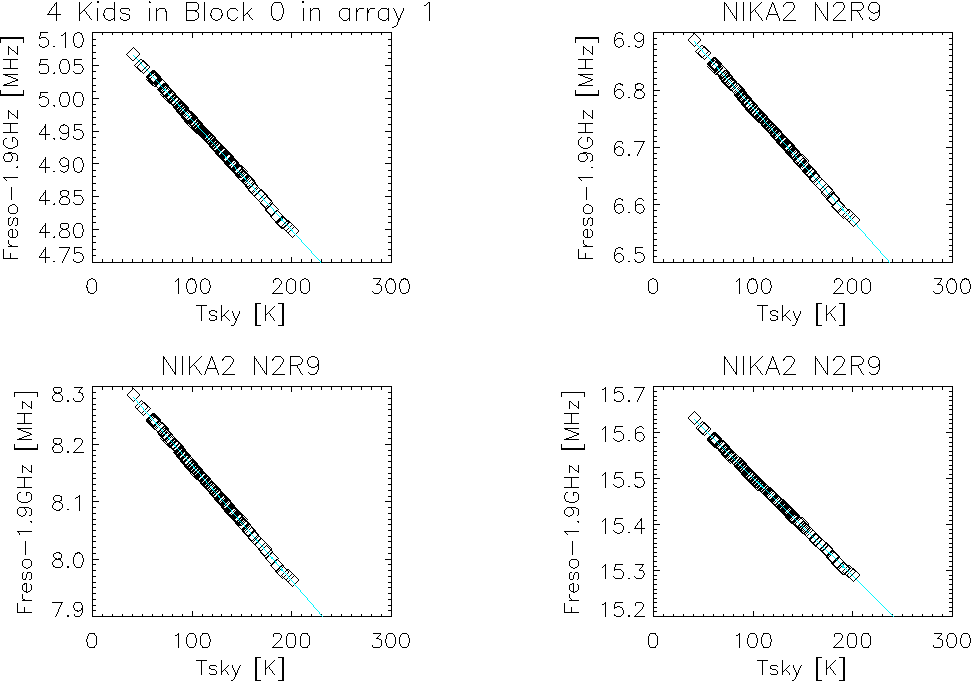
\includegraphics[trim={9cm 0cm 0cm 6.5cm}, clip=true, width=0.5\linewidth]{Figures/NIKA2/test_allskd4_N2R9v5_5-crop.pdf}
\caption[]{Exemple de la calibration de la réponse d'un KID à
  l'atmosphère. Chaque point (losange noir) représente la mesure de la
  fréquence de résonance du KID (par rapport à la valeur fixe de
  1,9\,GHz) pour l'un des paliers en élévation d'un scan de {\tt skydip}
  (Sect.~\ref{se:skydip}). Les points de mesures sont tracés en
  fonction de la température effective du ciel
  $T_{\rm{sky}} = T_{\rm{atm}}[1-e^{-\taunu\, x}]$ en Kelvin, où
  $\taunu$ est l'opacité atmosphérique telle qu'elle est ajustée. 
  La figure inclut les mesures réalisées à
  partir de 12 {\tt skydips} observés à des opacités atmosphériques
  $\taunu$ allant de 0,15 à 0,5 dans la bande à $1\,\rm{mm}$.
  La droite en bleu indique le meilleur ajustement du modèle donné à
  l'Eq.~\ref{eq:skydip}.}
\label{fig:skydipfitexample}
\end{center}
\end{figure}
%

\subsection{Tests des mesures d'opacité atmosphérique}
\label{se:opacity_tests}

Nous effectuons plusieurs tests de cohérence de l'estimation de
l'opacité atmosphérique. Tout d'abord, nous comparons les mesures
d'opacité obtenues avec les deux méthodes considérées, l'interpolation
au moment du scan des mesures du tau-mètre, $\tau_{225}$, et la mesure
dans les données brutes après calibration sur les {\tt skydips},
$\tau_{skydip}$, et ce, pour des observations réalisées au cours des
trois campagnes de référence. Les résultats sont présentés dans le
panel a) de la figure~\ref{fig:skydip-to-taumeter-correl}. La
corrélation entre les deux jeux de mesures de l'opacité reste stable
pour les trois campagnes d'observation. Cette stabilité entre les
résultats de deux méthodes indépendantes est une indication de la
robustesse de nos estimations de $\taunu$. Par ailleurs, nous
calculons une corrélation théorique entre $\tau_{skydip}$ et
$\tau_{225}$ en utilisant le modèle d'atmosphère ATM décrit
dans~\citet{Pardo2001}, les bandes passantes de NIKA2 telles qu'elles
ont été mesurées en laboratoire (Sect.~\ref{se:bandpass}) et une
étroite gaussienne centrée à 225\,GHz. Ces prédictions sont
représentées par les droites en noir à la
figure~\ref{fig:skydip-to-taumeter-correl}. Elles constituent un bon
modèle des corrélations mesurées à 1\,mm, mais tendent à sous-estimer
$\tau_{skydip}$ à 2\,mm. Cette différence peut avoir plusieurs
origines (erreur systématique dans les mesures de bande passante,
effet de la raie d'oxygène, etc.) mais n'a pas d'impact sur les
mesures de flux, puisque la calibration n'utilise ni modèle ATM, ni
les mesures des bandes passantes. Néanmoins, il est utile d'en garder
une trace afin de réitérer le test une fois qu'auront été effectuées
les mesures des bandes passantes de NIKA2 prévues au télescope de
30-m.
%
\begin{figure}[!thbp]
  \begin{center}
    \begin{overpic}[clip=true, trim={0, -0.3cm, -0.3cm, 0}, width=0.3\textwidth]{Figures/NIKA2/Opacity_correl_skydip_vs_tau_a1.pdf}
      \put(0,70){\footnotesize a)}
    \end{overpic}
    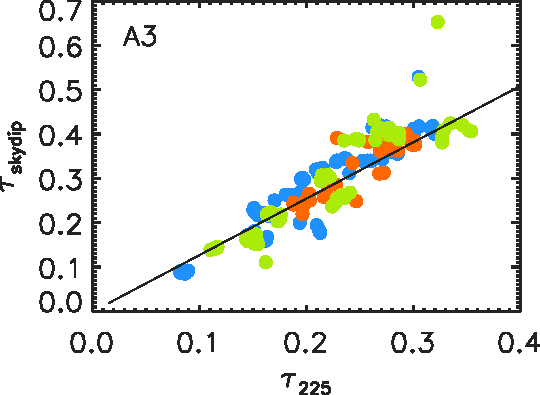
\includegraphics[clip=true, trim={0, -0.3cm, -0.3cm, 0}, width=0.3\textwidth]{Figures/NIKA2/Opacity_correl_skydip_vs_tau_a3.pdf}
    \begin{overpic}[clip=true, trim={-0.3cm, -0.3cm, 0, 0}, width=0.3\textwidth]{Figures/NIKA2/Opacity_skydip_to_taumeter_vs_elev_1mm.pdf}
      \put(0,70){\footnotesize b)}
    \end{overpic}
    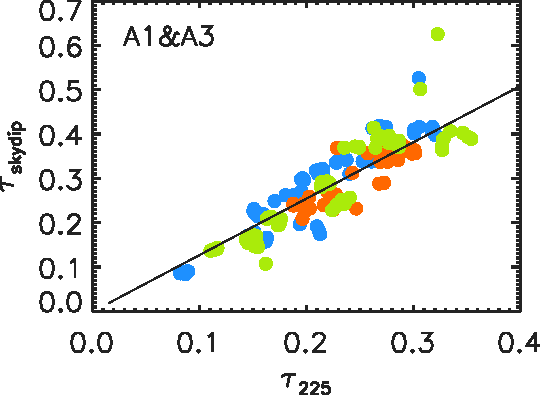
\includegraphics[clip=true, trim={0, -0.3cm, -0.3cm, 0}, width=0.3\textwidth]{Figures/NIKA2/Opacity_correl_skydip_vs_tau_1mm.pdf}
    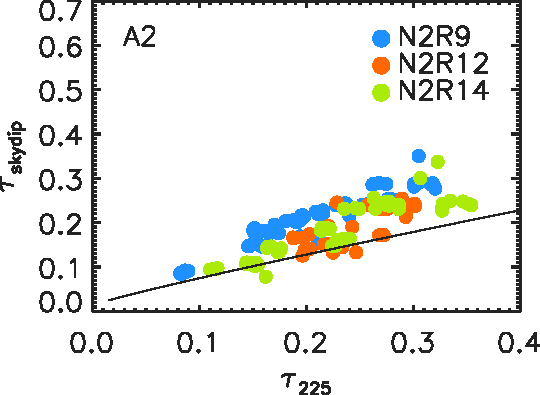
\includegraphics[clip=true, trim={0, -0.3cm, -0.3cm, 0}, width=0.3\textwidth]{Figures/NIKA2/Opacity_correl_skydip_vs_tau_a2.pdf}
    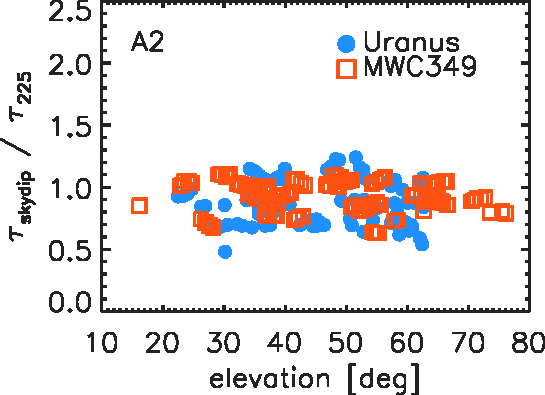
\includegraphics[clip=true, trim={-0.3cm, -0.3cm, 0, 0}, width=0.3\textwidth]{Figures/NIKA2/Opacity_skydip_to_taumeter_vs_elev_a2.pdf}
   \caption[]{Tests cohérence et de stabilité des estimations de
     l'opacité atmosphérique au zenith $\taunu$. a) Comparaison de
     $\taunu$ mesuré par NIKA2 après calibration avec les {\tt
       skydips}, noté $\tau_{\rm{skydip}}$, et de l'opacité mesuré par
     le tau-mètre à 225\,Ghz après interpolation au moment du scan et
     filtrage, $\tau_{225}$. La correlation $\tau_{\rm{skydip}}$ -
     $\tau_{225}$ est tracée pour une série de scans de calibrateurs
     observés lors des trois campagnes de référence. Un modèle de
     corrélation obtenu en intégrant un modèle ATM dans les bandes
     passantes de NIKA2 est aussi montré en noir à titre indicatif.  
     b) Le rapport $\tau_{\rm{skydip}}$ sur $\tau_{225}$ est tracé
     pour une large gamme d'élévation, à partir d'une série
     d'observations d'Uranus (points bleus) et du calibrateur
     secondaire MWC349 (carrés rouge).} 
\label{fig:skydip-to-taumeter-correl}
\end{center}
\end{figure}
%
Ensuite, nous testons une éventuelle dépendance de l'opacité
atmosphérique au zenith $\taunu$ avec la masse d'air $x$. Nous
calculons le rapport entre $\tau_{skydip}$ et $\tau_{225}$, définis
comme précédemment, et le traçons en fonction de l'élévation pour une
série de scans vers Uranus et vers un calibrateur secondaire
(MWC349). Les résultats sont présentés au panel b) de la
figure~\ref{fig:skydip-to-taumeter-correl}. Le rapport des mesures
d'opacité est stable pour une large gamme d'élévation allant de 15 à
$75\degree$. Cette stabilité est observée aussi bien pour les scans
d'Uranus, incluant plusieurs {\tt beammaps}, que pour les scans plus
courts vers MWC349. Ces tests indiquent la robustesse des estimations
d'opacité à l'élévation auxquelle est effectuée les observations et
aux types d'observation. 

Un ultime test de cohérence consistera à démontrer la stabilité des
flux mesurés après correction de l'atténuation de l'atmosphère à
partir de l'estimation de $\taunu$. Ce test sera présenté à la section
suivante (Sect.~\ref{se:calibration}). 



%----------------------------------------------------------------------------------------
%
%
%
%
%
%                 Calibration
%
%
%
%----------------------------------------------------------------------------------------
\section{Calibration absolue et relative}
\label{se:calibration}

Forts d'une reconstruction du plan focal, de la
caractérisation du lobe et de méthodes pour estimer l'atténuation de
l'atmosphère, nous avons tous les éléments en main pour réaliser la
calibration en flux. Pour cela, nous commençons par définir une
méthode de photométrie à la Sect.~\ref{se:systeme_photo}. Nous
effectuons une calibration relative entre les détecteurs, que nous
exploitons ensuite pour caractériser le plan focal à la
Sect.~\ref{se:gains}. Nous affinons l'estimation de l'opacité
atmosphérique à partir de tests photométriques à la
Sect.~\ref{se:corrected_skydip}. Nous résumons la méthode de
calibration \emph{baseline} à la Sect.~\ref{se:baseline_calibration}
et nous discutons une calibration alternative à la
Sect.~\ref{se:afternoon_calibration}.
        
\subsection{Système photométrique}
\label{se:systeme_photo}

\subsubsection{Le système de référence}

Notre photométrie procède de deux choix méthodologiques qui se fondent
sur des critères de simplicité et de robustesse. Tout d'abord, nous
mesurons les densités de flux à une fréquence fixe, $\nu_0$, choisie
arbitrairement, proche du centre de chaque bande passante. Ainsi,
$\nu_0 = 150$\,GHz dans la bande à 2\,mm et $\nu_0 = 260$\,GHz à
1\,mm. Modélisant la densité de flux d'un calibrateur primaire
$\rm{c}$ par $S_{\rm{c}} (\nu) = S_{\rm{c}} (\nu_0)\, f(\nu/\nu_0)$,
où $f(\nu/\nu_0)$ capture la dépendence spectrale, nous calibrons nos
densités de flux par rapport à $S_{\rm{c}} (\nu_0)$, sans intégration
dans les bandes passantes. Ces dernières n'étant utilisées que pour le
calcul des corrections de couleur, la propagation de leurs
incertitudes au flux mesuré est limitée pour la plupart des sources.
%
\begin{table}[!htbp]
\caption{Système photométrique de référence}
\label{tab:definitions}
\centering     
\begin{tabular}{lcc}
\hline\hline
      \noalign{\smallskip}
      & 1 mm & 2 mm \\
      \noalign{\smallskip}
      \hline
      \noalign{\smallskip}
      Fréquence de référence, $\nu_{0}$ & 260 GHz & 150 GHz \\
      FWHM de référence,  FWHM$_{0}$    & 12.5'' & 18.5'' \\
      \noalign{\smallskip}
      \hline
\end{tabular}
\end{table}
%

Le deuxième choix concerne la modélisation du lobe pour la mesure du
flux des sources ponctuelles. Comme présenté à la
Sect.~\ref{se:beam}, le lobe présente une structure complexe, avec
des lobes secondaires qui peuvent être asymétriques pour certaines
observations. L'ajustement de modèles complexes 2D (un template du
lobe) ou 1D (un profil) a été envisagé (et testé). Il s'accompagne
toutefois de difficultés, telles la dépendence aux conditions
d'observation (par exemple, la focalisation du télescope) et au
rapport signal-sur-bruit des données, qui détermine le niveau de
significance de la mesure des lobes secondaires. En revanche, nous
avons vérifié, sur des simulations et sur les données, qu'un modèle
simple du lobe assure une bonne stabilité des mesures de densité de
flux. Nous modélisons les cartes d'une source ponctuelle par une gaussienne
de référence dont la largeur à mi-hauteur (FWHM) est fixée à 
12,5'' à 1\,mm (260\,GHz) et de 18,5'' à 2\,mm (150\,GHz), soit
sensiblement plus grandes que la FWHM du lobe principal. La densité de
flux des sources correspond à l'amplitude de la gaussienne de
référence pour chacune des cartes. Les valeurs de référence FWHM$_0$ ont
été optimisées pour NIKA de façon à assurer la robustesse des mesures
des flux à l'effet des lobes secondaires. Nous avons vérifié cette
robustesse pour NIKA2 et nous avons aussi testé la stabilité des
mesures de flux pour des choix de FWHM$_0$ légèrement différents. Ces
deux choix, $\nu_0$ et FWHM$_0$, définissent notre système
photométrique et sont résumés dans la table~\ref{tab:definitions}.

\subsubsection{La calibration absolue}
Notre calibrateur primaire principal est la planète géante
Uranus. Neptune est parfois également utilisée dans les cas où Uranus
n'est pas observable dans des conditions optimales. Les densités de
flux attendues pour les deux planètes géantes sont calculées à partir
des modèles basées sur~\citet{Morenothesis}, tels qu'ils sont fournis par
l'ESA, et utilisés pour la calibration du satellite
\emph{Herschel}~\citep{Bendo2013}. La calibration absolue est réalisée
en ajustant l'amplitude $A_{\rm{c}}(\nu)$ d'une gaussienne de largeur
fixée à FWHM$_0$ dans les cartes produites pour chaque matrice $\nu$,
à partir d'une observation de l'un des calibrateurs primaires
$\rm{c}$. Les coefficients de calibration absolue pour les matrices
$\nu$ sont de la forme $S_{\rm{c}}(\nu_0) / A_{\rm{c}}(\nu)$. Les
cartes sont alors calibrées en Jy/beam. Par conséquent, les densités
de flux d'une source ponctuelle sont mesurées à partir des cartes dans
les bandes $\nu$ en 1) ajustant l'amplitude de la gaussienne de
référence dans chacune des cartes et 2) en applicant les corrections
de couleur comme détaillé dans~\citet{Perotto2019}.

\subsubsection{Le flux des sources diffuses}

Pour l'études des sources diffuses, les cartes calibrées en Jy/beam
doivent être corrigées de l'angle solide du lobe total, dont une
estimation est donnée à la Sect.~\ref{se:mainbeam}. Dans
\citet{Perotto2019}, nous distinguons deux corrections. Tout d'abord,
les cartes sont exprimées en Jy/sr en normalisant par l'angle solide soutendu
par la gaussienne de référence, $\Omega_0 = 2\pi \, \sigma_0^2$, avec
$\sigma_0 = 1/(2\sqrt{2 \log{2}})\, \rm{FWHM}_0$. Puis, nous prenons
en compte la fraction de flux contenue dans le lobe total en
corrigeant par l'efficacité de la gaussienne de référence, définie par
$\rm{BE}_{0}$ $=$ $\Omega_{0}$ $/$ $\Omega_{\rm{tot}}$.
L'estimation de l'efficacité
de référence utilise l'évaluation des différentes contributions à
$\Omega_{\rm{tot}}$, comme décrit à la
Sect.~\ref{se:beam}. L'efficacité de référence et les facteurs
correctifs à appliquer en fonction de l'étendue de la source
considérée, sont fournis dans~\citet{Perotto2019}.


\subsection{Les gains des détecteurs}
\label{se:gains}

En pratique, les calibrations relative et absolue sont réalisées
conjointement par l'estimation des gains des détecteurs lors de
l'analyse d'une {\tt beammap} vers un calibrateur primaire. Comme
décrit à la Sect.~\ref{se:FOV_geometry}, dans une procédure de
reconstruction du plan focal, les données brutes en Hz sont projettées
pour construire des cartes individuelles par KID pour chaque
matrice. L'amplitude de la gaussienne de
référence $A_k(\nu)$ est ajustée sur la carte du KID $k$ pour la
matrice $\nu$. Les gains des KID sont définis par
\begin{equation}
  G_k(\nu) = \frac{S_{\rm{c}}(\nu_0)\, e^{-\taunu\,x}}{A_k(\nu)},
  \label{eq:kid_gain}
\end{equation}
et correspondent donc aux coefficients de calibration à opacité
atmosphérique nulle, exprimés en Jy/Hz/beam. L'application de ces
coefficients aux TOI de chaque KID consiste bien en une calibration
absolue et relative.


Cette calibration repose sur l'analyse d'un seul scan. Pour améliorer
la précision de la calibration absolue, nous estimons un coefficient
correctif à partir d'une série de scans d'Uranus acquis tout au long
de la campagne d'observation. Ce coefficient est la moyenne sur tous
les scans des rapports flux attendu sur flux mesuré dans chacun des
scans.

Si les gains des KID, définis à l'Eq.~\ref{eq:kid_gain}, sont calculés
à des fins de calibration, leur distribution dans le champ de vue offre
une caractérisation intéressante des matrices de détecteurs. En effet,
le gain de chaque détecteur réalise un échantillonnage dans le champ
de vue de la réponse de NIKA2 à une source ponctuelle située en champ lointain, le
\emph{main beam flat field}. Nous traçons les \emph{flat fields} des
trois matrices à la figure~\ref{fig:avg_mbff}. Ils ont été construits
en moyennant les gains relatifs mesurés sur une série de cinq
{\tt beammaps} observées lors des deux dernières campagnes
techniques. Les gains relatifs correspondent aux gains normalisés par
le gain moyen pour tous les détecteurs d'une matrice. 
 % 
\begin{figure}[!thbp] 
\begin{center}
  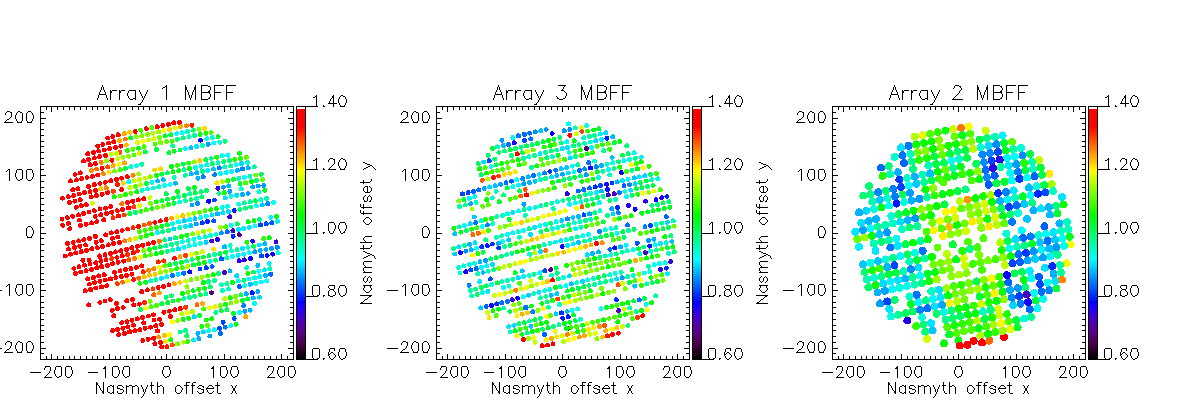
\includegraphics[width=0.95\textwidth]{Figures/NIKA2/Average_main_beam_flat_field_N2R9_10.png}
  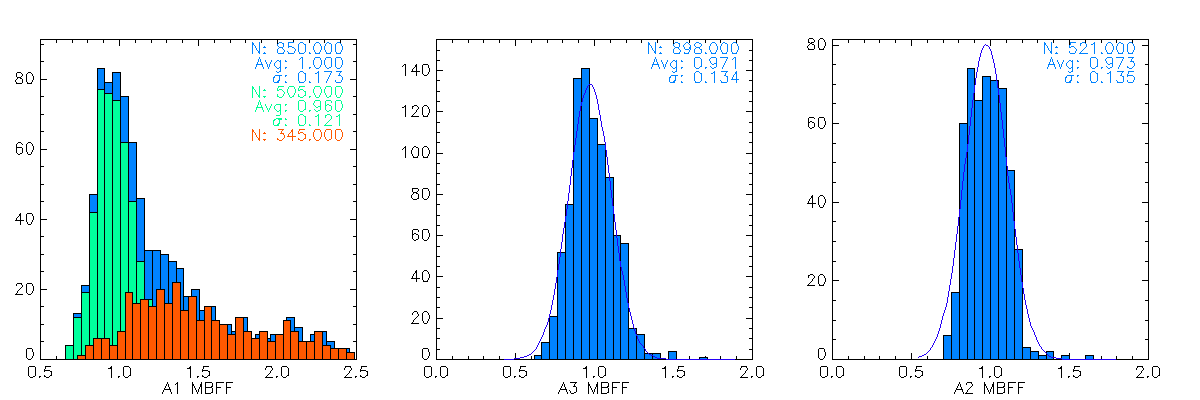
\includegraphics[width=0.8\textwidth]{Figures/NIKA2/Histo_average_main_beam_flat_field_N2R9_10.png}
  \caption[Average main beam flat fields]{\emph{Main Beam Flat
      Fields}. En haut, la distribution dans le champ de vue des gains
    relatifs des KIDs des matrices A1, A3 et A2. Les points indiquent
    la position de chaque détecteur par rapport au centre de la
    matrice, mesurée en secondes d'arc en coordonnées Nasmyth. Le code
    de couleur représente l'amplitude des gains relatifs, calculés
    suivant Eq.~\ref{eq:kid_gain} et normalisés par le gain moyen des
    détecteurs d'une matrice. En bas, les histogrammes des gains
    relatifs pour chaque matrice calculés en incluant soit tous les KIDs
    (en bleu), soit uniquement les KID du tiers gauche de la matrice
    A1 (rouge), soit uniquement les KID en dehors de ce tiers gauche
    (vert).}
 \label{fig:avg_mbff}
\end{center}
\end{figure}
%
Pour les matrices A3 et A2, les variations de gain sont d'amplitudes
faibles (rms d'environ $15\%$) et se répartissent dans le plan
focal suivant des structures pouvant être reliées à la connection des
KID aux lignes de base de l'électronique de lecture. En revanche, pour
la matrice A1 nous observons une variation des gains de forte
amplitude, affectant environ un tiers des KIDs situés dans un
croissant à gauche de la matrice. Les distributions des gains relatifs
pour chaque matrice sont présentées en bas de la
figure~\ref{fig:avg_mbff}. La distribution pour A1 est
significativement élargie, et cet élargissement est dù aux gains des
détecteurs situés dans le tiers gauche du champ de vue. Les KIDs de
cette zone, qui pour un même signal (Jy) ont une réponse en Hz
moindre, semblent obscursient. Par ailleurs, nous avons vérifié que cet
effet était également observé dans les \emph{flat fields} en champ
proche, en étudiant la réponse des KID à l'atmosphère, ce qui exclut
une origine liée au seul lobe principal.

Comme décrit à la Sect.~\ref{se:commissioning}, cet effet a été
observé pour la première fois après l'intervention sur l'instrument de
septembre 2016, au cours de laquelle la lame dichroïque, qui
présentait un défaut de planéité, avait été remplacée. De plus,
l'effet est bien reproduit par les simulations optiques incluant
un défaut de transmission de la lame dichroïque de l'une des composantes de
polarisation dans la bande à 1\,mm. Cette hypothèse a été directement
vérifiée en septembre 2018, par l'installation d'une troisième version
de la lame dichroïque, basée sur la technologie de la première version
(avant septembre 2016) et munie d'un support renforcé. Suite à cette
intervention, l'effet affectant le \emph{flat field} de A1 a bien
disparu, mais les défauts qui avaient motivés le remplacement de la
première génération de dichroïque sont réapparus. La lame dichroïque
de deuxième génération a été ré-installée pour revenir à la
configuration instrumentale post-septembre 2016. Ce défaut
de transmission de la composante de polarisation illuminant A1 a des
répercutions sur la sensibilité de cette matrice, comme discuté plus
avant à la Sect.~\ref{se:sensibilite}.      


\subsection{Tests photométriques de la correction de l'atmosphère}
\label{se:corrected_skydip}

Nous validons la calibration par des tests photométriques sur des
calibrateurs secondaires. Plusieurs sources de calibration sont
régulièrement suivies avec NIKA2, incluant des étoiles brillantes
(comme CRL2688), des nébuleuses planétaires faiblement résolues
(telles NGC7027). Parmi ces calibrateurs, le système d'étoiles binaire
MWC349~\citep{Tafoya2004} bénéficie de la prédiction la plus fiable du
flux attendu aux fréquences de NIKA2. En effet, pour cette source,
nous disposons d'observations effectuées à l'interféromètre du Plateau
de Bure (PdBI) et au \emph{Very Large Array} (VLA), permettant une
mesure précise de sa SED. Par ailleurs, l'incertitude liée aux
variabilités des calibrateurs secondaires est minimale pour MWC349,
car nous bénéficions d'un suivi régulier de cette source avec NOEMA,
pour lequel elle est un calibrateur. Cet exemple de synergie entre les
deux observatoires de l'IRAM a vocation à se développer. Pour finir,
MWC349 est une source ponctuelle pour le télescope de 30-m.

\`A partir de séries de scans OTF de $8' \times 5'$ vers MWC349
observés lors des trois campagnes de référence, nous testons la
stabilité des densités de flux mesurées aux conditions
atmosphériques. En particulier, nous testons les deux méthodes de
correction de l'opacité de l'atmosphère présentées à la
Sect.~\ref{se:opacity}. La figure~\ref{fig:mwc349_obstau_others}
montre le rapport flux mesuré sur flux attendu pour MWC349 en fonction
de la transmission atmosphérique sur la ligne de visée,
$\exp{(-\taunu \, x)}$. Cette figure inclut 72 scans sélectionnés sur
les critères \emph{baseline} (Sect.~\ref{se:scan_selection}). Dans les
panels du hauts, étiquetés \emph{taumeter}, la correction de
l'atténuation de l'atmosphère utilise les estimées de $\taunu$ issues
des mesures du tau-mètre à 225\,GHz
(Sect.~\ref{se:opacity_methods}). Dans les panels centraux, notés
\emph{skydip}, $\taunu$ est estimé via la calibration sur
les {\tt skydips} de NIKA2 (Sect.~\ref{se:opacity_methods}).  
%
\begin{figure}[!thbp]
  \begin{center}
    \begin{overpic}[clip=true, trim={0.9cm, 0.2cm, 0, 0.6cm},width=0.505\linewidth]{Figures/NIKA2/plot_flux_density_ratio_MWC349_obstau_tau225_narrow_1mm.pdf}
      \put(20,60){\footnotesize {\tt Taumeter}}
    \end{overpic}
    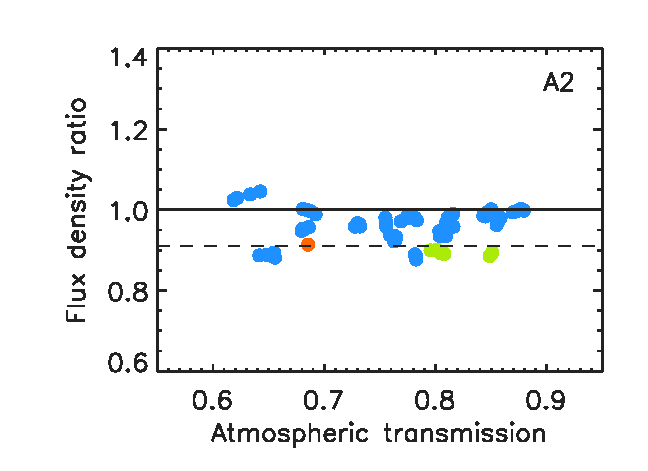
\includegraphics[clip=true, trim={1.8cm, 0.2cm, 0.5cm, 0.7cm},width=0.434\linewidth]{Figures/NIKA2/plot_flux_density_ratio_MWC349_obstau_tau225_narrow_a2.pdf}
    \begin{overpic}[clip=true, trim={0.9cm, 0.2cm, 0, 0.6cm},width=0.505\linewidth]{Figures/NIKA2/plot_flux_density_ratio_MWC349_obstau_skydip_narrow_1mm.pdf}
      \put(20,60){\footnotesize {\tt Skydip}}
    \end{overpic}
    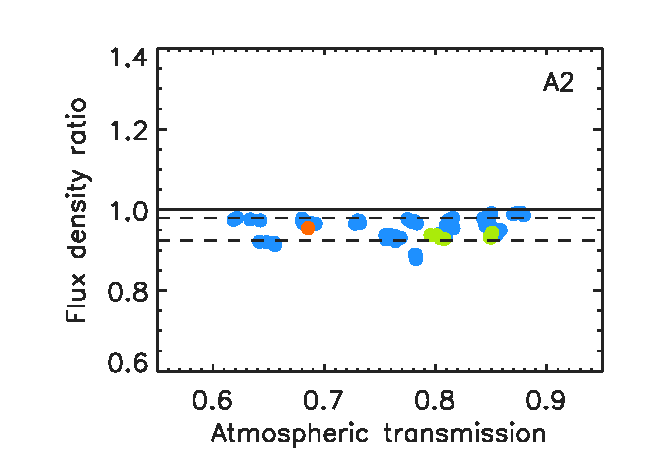
\includegraphics[clip=true, trim={1.8cm, 0.2cm, 0.5cm, 0.7cm},width=0.434\linewidth]{Figures/NIKA2/plot_flux_density_ratio_MWC349_obstau_skydip_narrow_a2.pdf}
    \vspace{-0.3cm}
    \begin{overpic}[clip=true, trim={0.9cm, 0.2cm, 0, 0.6cm},width=0.505\linewidth]{Figures/NIKA2/plot_flux_density_ratio_MWC349_obstau_corrected_skydip_narrow_1mm.pdf}
      \put(20,60){\footnotesize {\tt Baseline}}
    \end{overpic}
    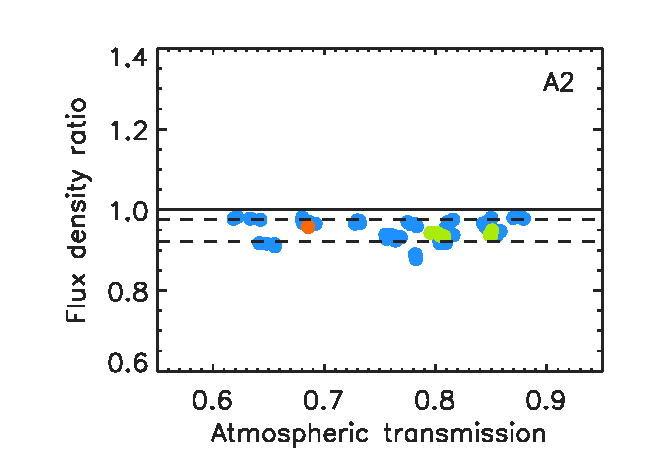
\includegraphics[clip=true, trim={1.8cm, 0.2cm, 0.5cm, 0.7cm},width=0.434\linewidth]{Figures/NIKA2/plot_flux_density_ratio_MWC349_obstau_corrected_skydip_narrow_a2.pdf}
    \caption[Calibration bias comparison]{Tests photométriques sur le
      calibrateur secondaire MWC349. Le rapport entre les densités de
      flux mesurées et attendues est tracé en fonction de la
      transmission de l'atmosphère, estimée par $\exp{(-\taunu x)}$,
      dans la bande à 1\,mm (à gauche) et à 2\,mm (à droite),   
      pour trois méthodes de calibration : en haut, label
      \emph{Taumeter}, $\taunu$ est estimé à partir des mesures du
      tau-mètre; au milieu, label \emph{Skydip}, l'estimation de
      $\taunu$ repose sur la calibration avec les \emph{skydips}; en
      bas, label \emph{baseline}, la méthode \emph{baseline} est
      utilisée. Les lignes pointillées correspondent à la rms des
      rapports de densité de flux.}
    \label{fig:mwc349_obstau_others}
  \end{center}
\end{figure}
%
Pour les deux méthodes, les flux mesurés sont en accord avec la
prédiction pour les trois campagnes d'observation et aux deux
fréquences. Le manque de flux de $5\%$ observé à 2\,mm reste
non-significatif, étant donné la précision de la prédiction du
flux. Pour \emph{taumeter}, les rapports de flux mesurés sont stables
dans toute la gamme de transmission atmosphérique testées, mais
présentent une plus grande dispersion que les rapports de flux
\emph{skydip}. Ce surcroit de dispersion est attendu étant donné que
l'opacité est estimée à l'azimuth fixe du tau-mètre et non à l'azimuth
du scan. Avec la méthode \emph{skydip}, nous observons un effet
systématique affectant les rapports de flux à 1\,mm, avec une
amplitude d'environ $15\%$ entre les
plus basses et les plus hautes transmissions atmosphériques. Cet effet
a motivé le recours à une correction des mesures d'opacité
\emph{skydip}.


\subsection{La méthode de calibration de référence}
\label{se:baseline_calibration}

Pour traiter l'atténuation des flux par l'atmosphère, la
calibration de référence, appelée \emph{baseline}, utilise une version
corrigée des opacités estimées avec la méthode de la calibration sur
les {\tt skydips} de NIKA2, que l'on notera
$\tau_{\rm{skydip}}$. Cette correction des $\tau_{\rm{skydip}}$
consiste en un facteur multiplicatif $a_\nu$ pour chaque matrice
$\nu$, qui est estimé à partir des densités de flux mesurées,
\begin{equation}
  S_\nu = \tilde{S}_\nu \,\,  e^{a_\nu \tau_{\rm{skydip}} x},
\end{equation}
sous une contrainte de stabilité dans la gamme de transmission
atmosphérique testée. Les facteurs $a_\nu$ modélisent la dégénérescence
entre $\taunu$ et $c_1$ dans l'ajustement de l'Eq.~\ref{eq:skydip}, en
particulier aux faibles opacités, où seule la quantité $c_1
T_{\rm{atm}} \taunu x$ est mesurée (voir Sect.~\ref{se:opacity_methods}). Nous
estimons les facteurs $a_\nu$ à partir de la série de 64 scans de
MWC349 observés durant le N2R9, puis nous verifions la stabilités des
flux mesurés pour cette source lors des deux autres campagnes
d'observation (N2R12 \& N2R14). Nous trouvons un facteur $a_\nu$
compatible avec l'unité à 2\,mm et valant environ 1,3 à 1\,mm. Par
ailleurs, nous vérifions que les facteurs correctifs additifs, dans un
modèle $a_\nu\tau_{\rm{skydip}} + b_\nu$, sont compatibles avec zéro. La
procédure et les résultats sont détaillés dans~\citet{Perotto2019}.

Les rapports entre les flux mesurés et les flux attendus de MWC349
lors des trois campagnes de référence sont tracés dans les panels du
bas de la figure~\ref{fig:mwc349_obstau_others}, notés
\emph{Baseline}. Les flux sont en accord avec les prédictions pour ces
trois campagnes d'observation et ils sont stables pour une large gamme de
transmissions atmophériques (0.5 à 0.9) dans les deux bandes de
fréquence.

En résumé, la calibration \emph{baseline} s'appuie sur les
méthodes suivantes : 1) les calibrations relative et absolue sont
réalisées dans le cadre du système photométrique de référence
(Sect.\ref{se:systeme_photo}), 2) l'atténuation atmosphérique est
compensée en utilisant les $\tau_{\rm{skydip}}$ corrigés et 3) l'effet
des variations journalières du lobe (Sect.\ref{se:fwhm_variations})
est minimisé en appliquant la sélection des scans \emph{baseline}
(Sect.\ref{se:scan_selection}). Cette calibration permet d'obtenir des
mesures de flux non-biaisées et robustes aux conditions atmosphérique
en préservant 16 heures d'observation par jour. Des méthodes de
calibration alternatives, visant à préserver les observations de
l'après-midi, sont discutées à la section suivante.

\subsection{Vers une méthode robuste aux variations du lobe}
\label{se:afternoon_calibration}

L'élargissement apparent des lobes, qui peut être observé lors du lever
du soleil et pendant l'après-midi, s'accompagne d'une variation des
densité de flux mesurées. Dans la calibration \emph{Baseline}, cet
effet est minimisé en excluant les huit heures d'observation les plus
impactées. Ici, nous discutons une méthode alternative visant à
inclure toutes les observations. L'idée consiste à mesurer
conjointement la densité de flux et la largeur du lobe afin
d'appliquer une correction photométrique pour compenser l'effet sur le
flux de l'élargissement du lobe. Une forme empirique simple pour cette
correction photométrique, dépendant uniquement de la FWHM du lobe au
premier ordre, est présentée dans~\citet{Perotto2019}. Le point
crucial est de mesurer précisément la FWHM du lobe même pour les
observations de sources diffuses ou faibles. Un tel suivi requiert des
observations dédiées, par exemple un scan OTF vers une source
ponctuelle brillante toutes les heures. Pour valider la méthode avant
une éventuelle mise en oeuvre d'observations dédiées, nous avons
proposé d'effectuer ce suivi des FWHM à partir des {\tt
  pointages}. Ces scans (Sect.~\ref{se:pointing}) sont effectués
environ toutes les heures, vers des sources ponctuelles brillantes;
comprenant quatres subscans de 10 secondes, ils permettent la
construction d'une carte, sur laquelle est ajustée la FWHM du
lobe. Toutefois, ce lobe ne correspond pas exactement au lobe de
NIKA2, puisque seuls les KID situés au centre des matrices observent
la source lors d'un {\tt pointage}. Finalement, la série temporelle
des FWHM issues des {\tt pointages} est filtrée et interpolée au
moment de l'observation de chaque scan. Nous avons vérifié que cette
méthode est efficace pour capturer l'évolution globale de la FWHM du
lobe (plus de détails dans~\citet{Perotto2019}).

Pour comparaison avec la calibration \emph{Baseline}, nous recalibrons
sans sélectionner les scans en fonction de l'heure d'observation et
en appliquant la correction photométrique aux densités de flux à
partir de la FWHM estimée par la méthode des {\tt pointages}. Cette
méthode de calibration alternative est appelée \emph{pointing-based
  photometric correction}, abrégée en \emph{PC-point}. Toujours avec
cette méthode, nous répétons les tests photométriques avec le
calibrateur secondaire MWC349. Le recours à la méthode \emph{PC-point}
permet d'inclure environ une vingtaine de scans supplémentaires par
rapport à la sélection \emph{baseline}. Les densités de flux mesurées
sont en accord avec les prédictions pour ce calibrateur et elles
restent constantes quelque soit la transmission atmosphérique. Ce test
constitue une première validation de la méthode \emph{PC-point}, ainsi
qu'un résultat encourageant pour la calibration des données affectées
par les variations journalières du lobe.



%----------------------------------------------------------------------------------------
%
%
%
%
%
%
%                LES INCERTITUDES
%
%
%
%
%----------------------------------------------------------------------------------------
\section{Incertitudes de calibration}

Nous évaluons l'incertitude sur les densités de flux en deux
temps. Tout d'abord, nous estimons la dispersion des mesures par
rapport à la moyenne, c'est-à-dire l'erreur RMS (\emph{root-mean
  square}), pour un large échantillon de données représentatif des
conditions d'observation rencontrées (Sect.~\ref{se:rms_error}). Cette
erreur englobe l'incertitude statistique ainsi qu'une partie des
effets systématiques résiduels dépendant des conditions
d'observation. Ensuite, nous évaluons les erreurs systématiques
non-liées aux conditions d'observation (Sect.~\ref{se:syste}).

\subsection{L'erreur RMS de calibration}
\label{se:rms_error}

Afin d'inclure un maximum d'observation des sources ponctuelles, y
compris celles dont le flux est peu connu, nous évaluons le rapport
entre la densité de flux mesurée sur un scan et la médiane des
densités de flux mesurées sur tous les scans de la source considérée.
Pour cela, la source doit être suffisament brillante pour permettre
une mesure significative du flux à partir d'un seul scan typique (OTF $5'
\times 8'$). En sus de la sélection de scan \emph{baseline}, nous
appliquons un seuillage tel que le flux des sources doit dépasser
800\,mJy à 1\,mm et 400\,mJy à 2\,mm. Nous disposons ainsi d'un jeu de
quelques centaines de scans de sources ponctuelles, que l'on note
\emph{PS-800mJy}. Ce jeu de scans
étant bien représentatif des conditions d'observation
rencontrées au téléscope de 30-m, l'étude de la distribution des
rapports flux mesuré sur médian nous permet d'estimer les incertitudes
de calibration d'origine optique, atmosphérique, et celles liées au
bruit instrumental et au bruit résiduel après traitement des données.

Pour caractériser la distribution des rapports de flux, nous évaluons
les intervalles de confiance à 68 et 95\%. Nous vérifions que la 
déviation standard des rapports de flux, notée $\sigma_\nu$, est
supérieure à l'intervalle à 68\% de niveau de confiance, nous
fournissant une estimation prudente de l'erreur à $1\,\sigma$. Ainsi,
nous utilisons $\sigma_\nu$ pour évaluer l'erreur de calibration RMS.

\begin{figure}[!thbp]
  \begin{center}
    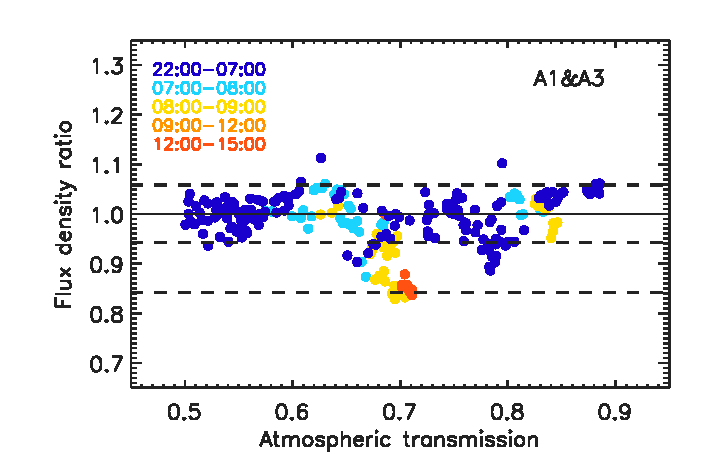
\includegraphics[clip=true, trim={0.9cm, 0, 0.5cm,
        0.6cm},width=0.45\linewidth]{Figures/NIKA2/plot_flux_density_ratio_obstau_allbright_obsdate_corrected_skydip_rescaled_1mm.pdf}
    \hfill
    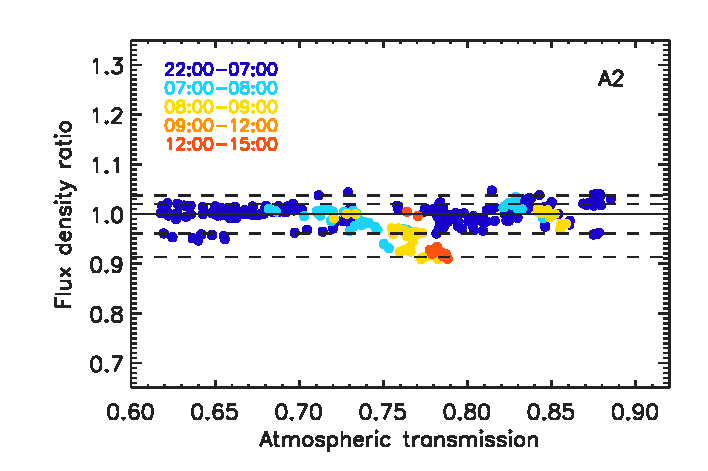
\includegraphics[clip=true, trim={0.9cm, 0, 0.5cm, 0.6cm},width=0.45\linewidth]{Figures/NIKA2/plot_flux_density_ratio_obstau_allbright_obsdate_corrected_skydip_rescaled_a2.pdf} 
    \caption[Baseline calibration rms error estimate]{Baseline
      rms calibration uncertainties. The
      measured-to-median flux density ratio of bright sources is
      plotted as a function of the atmospheric transmission
      color-coded according to the UT
      observation time of the scans for the combination of A1$\&$A3
      (top pannel)
      and for A2 (bottom pannel).
      The inner dashed lines from either sides of the
      unity-ratio line show the rms errors, which
      are less than 6\% at $1\,\rm{mm}$ and 3\% at $2\,\rm{mm}$, while
      the outer dashed lines show the $95\%$ confidence level contours.
      The lowest flux ratio data points correspond to some of the
      scans acquired during daytime between 8:00 UT and 15:00 UT
      hours (yellow and red), while the scans acquired during nighttime
      between 22:00 UT and 7:00 UT yield data points (dark blue)
      well distributed within the rms error with a few outliers.}
    \label{fig:allbright_rms_corrected_skydip}
  \end{center}
\end{figure}
%
\`A la figure~\ref{fig:allbright_rms_corrected_skydip}, nous
présentons les rapports de la densité de flux mesurée sur médiane,
après la calibration \emph{Baseline} et pour
le jeu de scans \emph{PS-800mJy} et testons leurs stabilités en
fonction de la transmission atmosphérique, $\exp{-\taunu x}$. Les
rapports de flux sont compatibles avec l'unité  dans l'intervalle de
transmission atmosphérique testé et dans les deux bandes de fréquence,
indiquant l'abscence d'effets systématiques significatifs après
correction de l'atténuation de l'atmosphère par la méthode décrite à
la Sect.~\ref{se:corrected_skydip}. Par ailleurs, nous observons un
groupe de scans pour lequel le rapport de flux est à la limite du
contour à 95\% de confiance. Un répérage des scans en fonction de
l'intervalle horaire auquel ils ont été observés (code de couleur)
nous indique que les scans concernés ont été observés soit le matin,
vers le lever du Soleil, soit en début d'après-midi, c'est-à-dire
proche des coupures sur l'heure UT, comme définies dans la sélection
\emph{Baseline}. Dit autrement, il serait possible de réduire encore
les incertitudes de calibration avec des coupures plus sévères, au
prix d'exclure davantage d'observations. Nous avons estimé que les
coupures \emph{baseline}, qui préservent 16 heures d'observation par
jour représentaient un bon compromis.

Dans la table~\ref{tab:Calibration_results_all}, nous rassemblons les estimations de l'erreur
de calibration RMS, basée sur $\sigma_\nu$, pour les différentes
méthodes de calibration discutées.
\begin{table*}[!htbp]
\begin{center}
\caption[Comparison of calibration results using three
  methods]{Erreur de calibration RMS en $\%$ pour trois méthodes de
  calibration : la méthode \emph{Baseline}
  (Sect.~\ref{se:corrected_skydip}), une méthode utilisant les opacités
atmosphériques dérivées des mesures du tau-mètre (Sect.~\ref{se:opacity_methods}) et une méthode utilisant une
correction photométrique (Sect.~\ref{se:afternoon_calibration}). La
première ligne indique le nombre de scans sélectionnés pour évaluer
les erreurs.} 
\label{tab:Calibration_results_all}
\begin{tabular}{lrrr}
  \hline\hline
  \noalign{\smallskip}
  \multicolumn{1}{c}{}  &  \multicolumn{3}{c}{Methods} \\\cline{2-4}
  \noalign{\smallskip}
  \multicolumn{1}{c}{Characteristics} &  \emph{baseline}  & {\small {\tt taumeter}}  & {\small {\tt PC-point}} \\
  \hline
  \noalign{\smallskip}
  $\#$ selected &   264    &    264   &  283 \\
  1mm           &   5.7    &    7.9   &  4.9 \\
  2mm           &   3.0    &    3.8   &  2.4 \\
\hline
\end{tabular}
\end{center}
\end{table*}

La méthode \emph{Baseline}, telle qu'elle est décrite à la
Sect.~\ref{se:corrected_skydip}, permet une mesure des densités de
flux avec une incertitude RMS $<6\%$ à 1\,mm et de $3\%$ à 2\,mm. Ce
résultat est remarquable pour une expérience millimétrique au sol,
pour lesquelles l'état de l'art de l'erreur RMS de calibration est
$\lesssim$ $10\%$ ~\citep{Dempsey2013_SCUBA2}. Il constitue une
validation de nos choix méthodologiques. La robustesse de la méthode
est également testée en comparant les résultats obtenus avec les méthodes
alternatives. Nous vérifions que la méthode \emph{Taumeter} est
associée à une dispersion légèrement supérieure des mesures de flux,
comme attendu (voir
Sects.~\ref{se:opacity_methods}~et~\ref{se:corrected_skydip}). En
revanche, la méthode \emph{PC-point} permet d'obtenir une erreur RMS
inférieure à l'erreur mesurée avec la méthode \emph{Baseline} tout en
incluant plus de scans. C'est un résultat encourageant pour les
méthodes fondées sur une correction photométrique. Toutefois, la
validation de telles méthodes requièrerait encore de s'assurer du
contrôle des effets systématiques liés à l'estimation de
l'élargissement apparent du lobe (qui est réalisée par un suivi de la
FWHM sur les {\tt pointages} dans le cas de \emph{PC-point}). Au
contraire, les effets systématiques sont sous-dominants pour la
méthode \emph{Baseline}, comme discuté à la section suivante.

\subsection{L'incertitude de calibration absolue}
\label{se:syste}

L'erreur RMS constitue une estimation des incertitudes liées
aux conditions d'observation. Les erreurs de calibration incluent en
sus l'incertitude de calibration absolue et les erreurs
systématiques.  

Si l'incertitude sur la mesure des opacités
atmosphériques $\taunu$ est bien inclue dans l'erreur de calibration
RMS, l'incertitude sur le facteur correctif $a_\nu$ qui est appliqué
aux estimées de $\taunu$ contribue à l'erreur systématique. Nous
propageons l'incertitude sur $a_\nu$, évaluée à $\Delta a_\nu = 0.03$,
à l'erreur sur le flux, pour deux valeurs de l'opacité atmosphérique
le long de la ligne de visée. Pour les conditions atmosphériques de
référence du télescope de 30-m de l'IRAM, définies par une hauteur
de vapeur d'eau saturante (pwv) de 2\,mm et une élévation de
$60\degree$, correspondant à de bonnes conditions lors des semestres
d'hier, nous trouvons une incertitude sur les flux inférieure au
pourcent dans les deux bandes de fréquence. Considérant les pires
conditions atmosphériques permises par la sélection de scan
\emph{Baseline}, l'erreur systématique sur les flux est au maximum de
$2\%$ à 1\,mm. De plus, ces erreurs sont évaluées pour le cas le plus
défavorable où la différence entre les conditions atmosphériques du
calibrateur primaire et de la source sont maximales. Elles représentent
des estimations pessimistes de l'erreur systématique liée à la
correction de $\taunu$.

Une autre source d'erreur systématique vient de la précision avec
laquelle sont connues les bandes passantes de NIKA2. Dans le cadre de
notre système photométrique, les densités de flux ne sont pas
intégrées dans les bandes passantes, mais données à une
fréquence de référence, ce qui minimise cette erreur
systématique. L'incertitude sur les bandes passantes se propage aux
flux uniquement pour les sources dont la densité spectrale d'énergie
diffèrent de celle du calibrateur primaire, via les corrections de
couleur. La caractérisation spectrale de NIKA2 en laboratoire à permis
une mesure des bandes passantes à mieux que 1\%. En utilisant cette
limite supérieure pour l'incertitude sur les bandes passantes, nous
trouvons une erreur sur les flux inférieure ou de l'ordre du pourmille
pour la plupart des sources. 

L'incertitude de calibration absolue est donc dominée par
l'incertitude sur le modèle de densité de flux pour notre calibrateur
primaire, Uranus, qui est estimée à environ $5\%$
dans~\citet{Bendo2013} aux fréquences d'observation de NIKA2. Nous
annonçons donc une erreur systématique négligeable et une incertitude
de calibration absolue de $5\%$ dans les deux bandes de fréquence.





%----------------------------------------------------------------------------------------
%
%
%
%
%
%               Sensibilité
%
%
%
%
%
%----------------------------------------------------------------------------------------
\section{Sensibilité}
\label{se:sensibilite}


Nous caractérisons la sensibilité de NIKA2 en évaluant la densité de
flux équivalente au bruit (\emph{Noise Equivalent Flux Density},
NEFD). La robustesse de cette évaluation est testée en comparant les
résultats de différentes méthodes et en utilisant un vaste jeu de
données. \`A la Sect.~\ref{se:nefd_methodes}, nous présentons deux
méthodes d'estimation de la NEFD et comparons les résultats pour un
même jeu de données. Ensuite, à la Sect.~\ref{se:nefd_mesures}, nous
étudions l'évolution de la NEFD avec les conditions atmosphériques et
discutons l'implication de la NEFD mesurée sur les temps d'observation
requis pour obtenir une cartographie à une profondeur donnée. 


\subsection{Méthodes}
\label{se:nefd_methodes}

La NEFD correspond à l'erreur à $1\,\sigma$ que l'on mesure sur la
densité de flux pour une seconde d'intégration sur la source et à une
opacité atmosphérique nulle. Elle est donc reliée à l'erreur à
$1\,\sigma$ sur la densité de flux, notée $\Delta S_\nu$,  par
\begin{equation}
  \Delta S_\nu (t) = {\rm{NEFD}} \,\, e^{ \tau_{\nu} x}
  \frac{1}{\sqrt{t_{\rm{det}}(t)}},
  \label{eq:relation_sigma_nefd}
\end{equation}
où $t_{\rm{det}}$ est le temps d'observation pendant lequel au moins un
détecteur pointe sur la source. Ce temps dépend de la stratégie de
balayage de la source. Il est égal au temps d'observation réel, $t$,
si la source ne sort à aucun moment du champs de vue et que celui-ci
est rempli de détecteurs valides.

Nous avons développé deux méthodes pour estimer la NEFD. L'une,
appelée \emph{Deep Integration}, se base sur l'étude de l'évolution du
bruit dans les cartes de densité de flux, lors d'une observation
longue d'une source faible, tandis que l'autre, \emph{Scatter}, repose
sur l'extrapolation à opacité nulle d'un ensemble de mesures de NEFD
sur des scans individuels.
Pour \emph{Deep Integration}, nous construisons une série de cartes de
la densité de flux à partir d'une longue observation d'une même source, en
incluant de plus en plus de scans. Chaque scan est utilisé pour
produire une carte individuelle comme décrit à la
Sect.~\ref{se:overview_pipeline}. Puis ces cartes par scan sont
pondérées par l'inverse de leur variance et co-additionnées pour
construire la carte finale. Leur contribution relative à la
co-addition va donc dépendre de l'atténuation de l'atmosphère au
moment du scan. Cet effet est pris en compte lors du calcul du temps
d'intégration par détecteur pour la co-addition de $n$ scans, en
définissant un temps d'intégration effectif, $t_{\rm{eff}} (n)$, qui
inclut l'atténuation de l'atmosphère. Avec cette définition, 
l'Eq.~\ref{eq:relation_sigma_nefd} se ré-écrit
$\Delta S_\nu (n) = {\rm{NEFD}} / \sqrt{t_{\rm{eff}}(n)}$.
L'évolution de $\Delta S_\nu$ avec le nombre de scan $n$ est mesurée
directement dans la série de cartes de densité de flux, et la NEFD est
estimée en ajustant un modèle en $t^{-1/2}$ sur ces mesures.

La seconde méthode, $\emph{Scatter}$, consiste à mesurer directement
la NEFD sur la ligne de visée, NEFD$_{\taunu x}$ = NEFD $\exp{ \tau_{\nu} x}$, à partir
d'une carte de la densité de flux, en inversant
Eq.~\ref{eq:relation_sigma_nefd}. La source ciblée doit être peu
brillante, $<1\,$Jy, pour éviter que l'estimation de lincertitude sur
le flux ne soit biaisée par le signal. En répétant une telle mesure
sur un grand nombre de scans acquis dans des conditions d'observation
diverses, nous pouvons vérifier l'évolution de la NEFD avec
l'atténuation atmosphérique. La NEFD est estimée en prenant la médiane
des mesures de la NEFD sur la ligne de visée, après correction de
l'atténuation de l'atmosphère.    

\begin{figure}[!thbp]
  \begin{center}
    \includegraphics[trim={0.5cm, 0, 0, 0.5cm}, clip, angle=0, width=0.495\textwidth]{Figures/NIKA2/hls_nefd_vst.eps}
    \includegraphics[trim={0.5cm, 0, 0.2cm, 0.5cm}, clip, angle=0, width=0.485\textwidth]{Figures/NIKA2/hls_NEFD_vs_TauElev_all.eps}
    \caption{Application de deux méthodes d'estimation de la NEFD à
      une longue observation de \hls. \`A gauche, l'erreur à 1\,$\sigma$
      sur la densité de flux est tracée en fonction du temps
      d'intégration effectif $t_{\rm{eff}}$ (voir le texte). Les
      droites en noir représentent les meilleurs ajustement d'un
      modèle en $t_{\rm{eff}}^{-1/2}$; leur amplitude donne une
      estimée de la NEFD. \`A droite, la NEFD mesurée sur
      la ligne de visée est tracée en fonction de l'opacité
      atmosphérique observée, $\taunu\,x$. Les courbes en noir
      montrent l'évolution attendue en $\exp{\taunu\,x}$, normalisée
      par la NEFD à atmosphère nulle. Dans les deux panneaux,
      l'analyse est effectuée pour la matrice  A1 (bleu clair), A3
      (bleu foncé), la combinaison A1\&A3 (bleu ciel), et A2 (rouge).}
    \label{fig:nefd_twomethods}
  \end{center}
\end{figure}
%
Nous comparons les résultats de ces deux méthodes sur un même jeu de
données à la Fig.~\ref{fig:nefd_twomethods}.
Pour cela, nous avons choisi une source assez faible,
\hls~\citep{Combes2012}, dont le flux attendu dans les bandes de NIKA2
est de quelques dizaines de mJy. Cette source a été observée en
effectuant des scans OTF $8' \times 5'$, pendant environ neuf heures,
lors de la campagne N2R9. Le panneau de gauche de la
Fig.~\ref{fig:nefd_twomethods} montre l'incertitude sur la densité
de flux en fonction du temps effectif d'intégration,
tandis que le panneau de droite présente la NEFD sur la ligne de
visée, NEFD$_{\taunu x}$, en fonction de l'opacité sur la ligne de
visée, $\taunu x$. Nous vérifions que l'incertitude sur le flux, pour
les matrices individuelles et pour la combinaison des matrices à 1\,mm,
diminue avec le temps d'intégration en $t^{-1/2}$ comme attendu. Nous
vérifions également l'évolution attendue de la NEFD$_{\taunu x}$ avec
l'atténuation de l'atmosphère. Finalement, les
estimées de la NEFD avec les deux méthodes, rassemblées dans la
table~\ref{tab:nefd_summary}, sont en accord à mieux que 7\%. Le
choix méthodologique a donc peu d'impact sur l'estimation de la
NEFD. Nous testons ensuite nos résultats et estimons les incertitudes
sur la NEFD en utilisant un plus grand jeu de données.  

%  comparison entre methods
\begin{table}[!htbp]
  \centering
  \caption[]{Tests de stabilité de la NEFD. Estimées de la NEFD
    en $\rm{mJy}.s^{1/2}$ obtenues en utilisant soit la méthode \emph{Deep
      Integration}, abrégée en Deep int., soit la méthode
    \emph{Scatter}, et pour deux jeux de données, l'observation longue de
    \hls\ et l'ensemble des scans vers des sources sub-Jy acquis lors
    des trois campagnes de référence. La dermière ligne du tableau
    donne les résultats pour la combinaison de tous ces scans (soit 202,
    481 et 430 scans lors de N2R9, N2R12 and N2R14, respectivement).}
  \label{tab:nefd_summary}
  \begin{tabular}{llrrrr}
    \hline\hline
    \noalign{\smallskip}
    Data set   & Method   & A1      &   A3    &   A1\&A3 &    A2 \\
    \noalign{\smallskip}
    \hline
    \noalign{\smallskip}
    \hls &     Deep int.  &  46.6  &    38.4  &    30.4  &   8.5  \\
    %   G2   &    $t^{-1/2}$  &  44.0  &    34.7  &    29.6  &  7.8  \\
         &     Scatter    &  45.7  &    36.3  &    28.5  &   8.2  \\
    \hline
    \noalign{\smallskip}
    N2R9     & Scatter    & 47.0 &  36.9  & 28.8  & 8.4 \\
    N2R12    &            & 47.3 &  36.4  & 30.2  & 8.5 \\
    N2R14    &            & 47.3 &  39.8  & 30.9  & 9.3 \\
    Combined &            & 47.2 &  37.9  & 30.1  & 8.8 \\
    \hline
  \end{tabular}
\end{table}

\subsection{Tests de robustesse aux conditions d'observation}
\label{se:nefd_mesures}

Nous utilisons la méthode \emph{Scatter}, qui est applicable à des
observations de sources variées, pour tester la robustesse de
l'estimation de la NEFD sur un vaste jeu de données. Ce jeu se compose
de l'ensemble des scans des trois campagnes de réference, vers des
sources de flux inférieur à 1\,Jy dans les deux bandes de fréquence,
et respectant les critères de sélection \emph{Baseline}. Il comprend
plus d'un millier de scans. \`A la
figure~\ref{fig:nefdvsbackground_below_1Jy}, nous traçons la NEFD sur
la ligne de visée, NEFD$_{\taunu x}$ , en fonction de l'opacité
atmosphérique observée, $\taunu x$, en distinguant les scans par
campagnes d'observation. Les courbes ne résultent pas de l'ajustement
d'un modèle mais représentent l'évolution attendue avec l'atténuation
de l'atmophère, normalisée par la NEFD à atmosphère nulle. Nous
vérifions ainsi que la NEFD$_{\taunu x}$ varie comme attendu avec le
"bruit du ciel'', pour une grande gamme de conditions d'observation. De
plus, nous mesurons des NEFD$_{\taunu x}$ compatibles pour les trois
campagnes de référence. Les valeurs de la NEFD estimées pour chaque
campagne et pour l'ensemble du jeu de données sont compilées dans la
Table~\ref{tab:nefd_summary}. Nous évaluons l'incertitude sur la NEFD
en calculant la rms des mesures de NEFD$_{\taunu x}$ corrigées de
l'atténuation de l'atmophère. Nous trouvons une erreur rms de
3\,mJy.s$^{1/2}$ à 1\,mm et 1\,mJy.s$^{1/2}$ à 2\,mm, en accord avec la
dispersion des estimées de la NEFD données à la
Table~\ref{tab:nefd_summary}. En utilisant l'estimation sur l'ensemble
des scans, nous annonçons une NEFD de $30 \pm 3$\,mJy.s$^{1/2}$ à 1\,mm
et de  $9 \pm 1$\,mJy.s$^{1/2}$ à 2\,mm. Par ailleurs, nous constatons
une moindre sensibilité de la matrice A1 comparée à A3, que nous
interprétons comme l'impact du défaut de transmission avéré de la lame
dichroïque (Sect.~\ref{se:gains}).
%
\begin{figure}[!thbp]
\begin{center}
  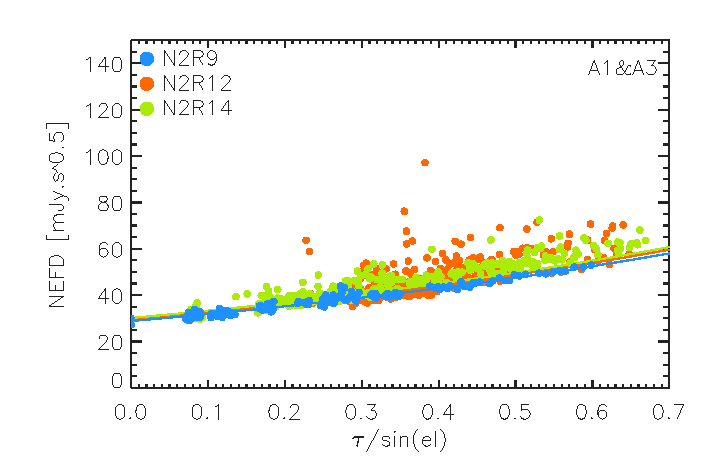
\includegraphics[clip=true,width=0.47\textwidth]{Figures/NIKA2/plot_nefd_vs_obstau_corrected_skydip_vfinal_1mm.pdf}
  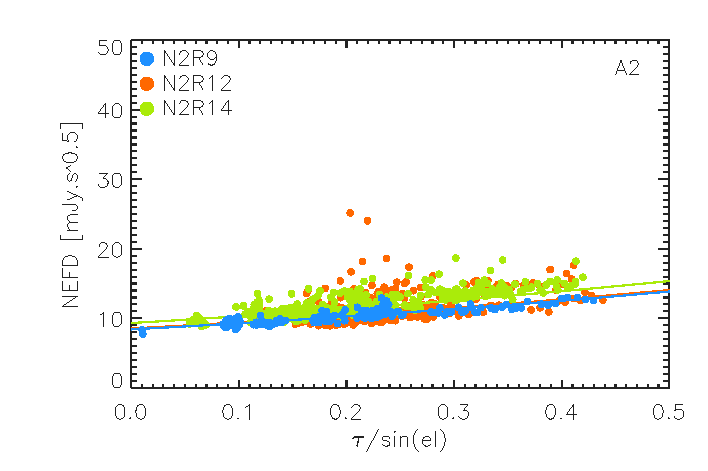
\includegraphics[clip=true,width=0.47\textwidth]{Figures/NIKA2/plot_nefd_vs_obstau_corrected_skydip_vfinal_a2.pdf}
  \caption{\'Evolution de la NEFD avec les conditions
    d'observation. La NEFD le long de la ligne de visée, NEFD$_{\taunu
    x}$, est tracée en fonction de l'opacité atmosphérique observée,
    $\taunu\,x$, dans la bande à $1\,\rm{mm}$ (à gauche) et à
    $2\,\rm{mm}$ (à droite). Les points de données correspondent aux
    estimées de NEFD$_{\taunu x}$ en $\rm{mJy}\cdot s^{1/2}$ obtenues
    lors des campagnes N2R9 (en bleu), N2R12 (orange) and N2R14
    (chartreuse). Les courbes représentent l'évolution attendue de la
    NEFD sur la ligne de visée en fonction du "bruit du ciel'',
    normalisée par l'estimée de la NEFD à atmosphère nulle.}
  \label{fig:nefdvsbackground_below_1Jy}
\end{center}
\end{figure}


Nous évaluons aussi la vitesse de cartographie (\emph{Mapping Speed}), 
définie comme la zone du ciel $\mathcal{A}_{\rm{scan}}$ qui peut être
observée à un niveau de bruit $\Delta_\sigma$ of $1\,\rm{mJy}$ en un
temps d'intégration $\Delta_t$ de une heure. En notant $d_{\rm{FOV}} =
6.5\,\rm{arcmin}$ le diamètre du champ de vue et $\eta$ la fraction de
KID valids (Sect.~\ref{se:fov_geometry}), la vitesse de cartographie
$M_{\rm{s}}$ s'écrit: 
\begin{equation}
M_{\rm{s}} = \frac{\mathcal{A}_{\rm{scan}}}{\Delta_\sigma\Delta_t} = 
\eta \, \frac{\pi}{4} d_{\rm{FOV}}^2 \, \frac{1}{\rm{NEFD}^2}\, ,
\label{eq:mapping_speed}
\end{equation}
et s'exprime en arcmin$^2 \cdot \rm{mJy}^{-2} \cdot
\rm{h}^{-1}$. C'est cette quantité qui est utilisée pour calculer
les temps d'observation. Ainsi, le temps d'observation nécessaire pour
atteindre le niveau d'incertitude sur les densités de flux
$\sigma_{obs}$ souhaité, sur une certaine couverture du ciel
$\mathcal{A}_{\rm{scan}}$, et en supposant une opacité atmosphérique
  sur la ligne de visée $\taunu x$ est
\begin{equation}
  t_{\rm{obs}} = \frac{\mathcal{A}_{\rm{scan}}}{ M_{\rm{s}}} \, \left(\frac{e^{\taunu\, x}}{\sigma_{obs}}\right)^2.
\end{equation}
\`A partir de l'estimation de la NEFD, nous dérivons une vitesse de
cartographie de $111 \pm 11$ et $1388 \pm 174$ arcmin$^2 \cdot
\rm{mJy}^{-2} \cdot \rm{h}^{-1}$ respectivement à 1 et
2\,mm. Ce résultat remarquable situe NIKA2 parmi les meilleurs
instruments millimétriques de cartographie haute-résolution d'un grand
champ de vue~\citep{Tony2019}.

